\documentclass[11pt,a4paper]{report}
\usepackage[pdftex]{hyperref}
\usepackage{mathtext}
\usepackage{cmap}
\usepackage[T2A]{fontenc}
\usepackage[utf8]{inputenc}
\usepackage[russian]{babel}
\usepackage{mathtools}
\usepackage{amsmath, amsthm,amsfonts,mathabx,amssymb,array,float,floatflt,titlesec,epigraph,indentfirst,graphicx,tabularx,subcaption}
\usepackage{wasysym,varwidth}
\DeclareUnicodeCharacter{1F600}{\smiley}
\usepackage[left=1.5cm,right=1.5cm,top=1.5cm,bottom=1.5cm,includefoot,footskip=0.5cm]{geometry}
\usepackage{tikz}
\usepackage{wrapfig}

\usepackage{enumitem}
\makeatletter
\AddEnumerateCounter{\asbuk}{\russian@alph}{щ}
\makeatother

\setlength{\parskip}{2pt}
\setlength{\intextsep}{4pt}

\titleformat{\section}{\centering\normalfont\bfseries}{}{1em}{}

\setlength\epigraphrule{0pt}
\setlength\epigraphwidth{.5\textwidth}

\newenvironment{prf}[1][\textbf{\textit{Решение}}]{\par\indent\pushQED{\qed}\itshape#1. \normalfont\ignorespaces}{\popQED}
\newenvironment{dok}[1][\textbf{\textit{Доказательство}}]{\par\indent\pushQED{\qed}\itshape#1. \normalfont\ignorespaces}{\popQED}
\newenvironment{prim}[1][\textbf{\textit{Примечание}}]{\par\indent\pushQED{\qed}\itshape#1. \normalfont\ignorespaces}{}
\newenvironment{samp}[1][\textbf{\textit{Пример}}]{\par\indent\pushQED{\qed}\itshape#1. \normalfont\ignorespaces}{}

\newtheoremstyle{myrmk}{3pt}{3pt}{\rmfamily}{\parindent}{\itshape}{.}{.5em}{}
\theoremstyle{myrmk}
\newtheorem{itm}{}[chapter]

\newtheoremstyle{mypln}{3pt}{3pt}{}{\parindent}{\bfseries}{.}{.5em}{}
\theoremstyle{mypln}
\newtheorem{thm}[itm]{Задача}
\newtheorem{prp}[itm]{Предложение}
\newtheorem{lem}[itm]{Лемма}

\newtheoremstyle{mydfn}{3pt}{3pt}{\rmfamily}{\parindent}{\bfseries}{.}{.5em}{}
\theoremstyle{mydfn}
\newtheorem{dfn}{Определение}
\newtheorem{ex}{Упражнение}
\newtheorem{prop}{Свойство} 
\newtheorem{thrm}{Теорема}

\newtheoremstyle{myques}{3pt}{3pt}{}{\parindent}{\bfseries}{.}{.5em}{}
\theoremstyle{myques}
\newtheorem{ques}{Контрольный вопрос}


	
\newcommand{\head}[2]
{\newpage
    \begin{minipage}[h]{0.1\linewidth}
        
\includegraphics[width=1\linewidth]{./img/logo}
    \end{minipage}
    \begin{minipage}{0.86\linewidth}
        \textbf{Творческая лаборатория <<ДваждыДва>> Спецматематика 8 класс #1}
    \end{minipage}
\begin{center}
	\textbf{#2}
\end{center}
\setcounter{footnote}{0}
}
 
\newcommand{\del}{\mathop{\raisebox{-2pt}{\vdots}}}
\newcommand{\ndel}{\mathop{\raisebox{-2pt}{\lefteqn{\vdots}}\setminus}}

\newcommand{\skdel}{\mathop{\raisebox{-2pt}{~\vdots~}}}
\newcommand{\nskdel}{\mathop{\raisebox{-2pt}{~\vdots~}}}

\newcommand{\makecircle}[2]{\tikz\draw[#1,fill = #2] circle (.5ex);} % шарик



 
\title{Курс спецматематики в листках для 8 класса}
\author{Автор: Иванова Елена Юрьевна\\
	Редактор: Кузнецов Глеб Михайлович\\
	Наборщик текста: Соколовский Всеволод Владимирович}

\date{\today}

\begin{document}
\maketitle
\tableofcontents
\newpage

\chapter{Логика}
\head{Сентябрь}{Листок 8. Логика. Теория.}

\textit{Логика} (от древнегреческого logos – слово, выражающее мысль) является началом любой научной теории. В древние века многие философы занимались поисками истины как таковой, изобретая системы аксиом и правила рассуждений. Наиболее известным до нас именем в этой области является Аристотель (384 - 322 гг. до н.э.). Именно Аристотель создал чистую систему силлогизмов– правил вывода, что и привело к возникновению теории логики.\footnote{Математическое исследование этих вопросов берет своё начало от основополагающего труда Джорджа Буля, изданного в Лондоне в 1854 году. Этот труд Буля положил начало математической логики, систематическое развитие
которой было достигнуто работами многих математиков XX века.}
\par
Основная функция логики как науки – изучение того, как из одних утверждений можно выводить другие. Многими правилами логики мы с детства пользуемся неосознанно. Определение, доказательство, опровержение и т.д. – все это функции логики. 
\par
Правила вывода позволяют преобразовывать исходные утверждения подобно тому, как тождественные преобразования в математике дают возможность решать различные системы уравнений. При этом предполагается, что вывод зависит только от способа связи входящих в него утверждений и их строения, а не от их конкретного содержания. Изучая, ''что из чего следует'', логика выявляет наиболее общие или, как говорят, формальные условия правильного мышления. Следующим шагом формализации логики является появление специальной символики для точной и компактной записи утверждений и определения операций над ними. Некоторые такие символы мы уже использовали, с другими символами мы познакомимся позже. 
\par
С появлением языка математической логики стало возможным составлять алгоритмы логического вывода. Стали вести речь о создании искусственного интеллекта. В последнее время логика находит все более широкое применение в технике при исследовании и разработке вычислительных машин, дискретных автоматов. Её методы используются в теории преобразования и передачи информации, теории вероятностей и комбинаторном анализе. Математическая логика находит своё применение в экономике, биологии, медицине, психологии, праве, языкознании.

Решение некоторых логических задач можно описать с помощью таблиц. Вы, скорее всего, уже знакомы с такими методами решения. При решении приходится рассматривать большое количество вариантов, перебирать различные случаи. При этом очень легко что-то потерять, забыть рассмотреть какой-то случай. Чтобы избежать всех этих проблем, математики придумали заносить результаты своих рассуждений в таблицы. Такой метод решения получил название табличной логики. Поясним, в чём заключается этот метод. Допустим, у нас есть три бумажные фигурки: круг, квадрат и треугольник. Они трёх разных цветов: синего, красного и жёлтого. Тогда мы можем нарисовать такую таблицу:

\begin{center}
\begin{tabular}{ | m{3cm} | m{3cm}| m{3cm} | m{3cm} | } 
  \hline
  & красный & синий & жёлтый \\ 
  \hline
  круг &    &   & \\ 
  \hline
  квадрат &    &   & \\ 
  \hline
  треугольник &    &   & \\ 
  \hline
\end{tabular}
\end{center}

Если нам даны ещё какие-то условия про эти фигурки, то мы можем начать расставлять ''плюсы'' и ''минусы'' в эту таблицу. ''Плюс'' означает, что данный вариант реализуется, ''минус'' означает, что не реализуется. Заметьте, что должны быть выполнены следующие условия:

\begin{enumerate}
    \item В каждой строке есть ровно один ''плюс''.
    \item В каждом столбце есть ровно один ''плюс''.
\end{enumerate}

Первое условие означает, что каждый предмет покрашен в один из указанных цветов. Второе – что есть ровно один предмет каждого цвета.

\newpage

\begin{thm}
    Четыре спортсменки – Аня, Валя, Галя и Даша – заняли первые четыре места в соревновании по гимнастике, причём никакие две из них не делили между собой эти места. На вопрос, какое место заняла каждая из спортсменок, трое болельщиков ответили:
    \par
    \textit{Первый:} Аня – второе место. Даша – третье место.
    \par
    \textit{Второй:} Аня – первое место. Валя – второе место.
    \par
    \textit{Третий:} Галя – второе место. Даша – четвёртое место.
    \par
    Оказалось, что каждый из болельщиков ошибся один раз.
    \par
    Какое место заняла каждая из спортсменок?
\end{thm}

\begin{prf}
    Поскольку мы не знаем точно, какое из двух утверждений каждого болельщика верно, а какое ложно, то рассмотрим утверждения первого болельщика и разберём два варианта.
    \par
    \textit{Первый вариант:} ''Аня заняла второе место'' – верно, а ''Даша заняла третье место'' – неверно. 
    \par
    Составим таблицу:
    \begin{center}
    \begin{tabular}{ | m{2cm} | m{2cm}| m{2cm} | m{2cm} | m{2cm} | } 
        \hline
        & 1 & 2 & 3 & 4 \\ 
        \hline
        Аня & -- & + & -- & --\\ 
        \hline
        Валя &  & -- &   &   \\ 
        \hline
        Галя &  & -- &   &   \\ 
        \hline
        Даша &  & -- & -- &   \\ 
        \hline
    \end{tabular}
    \end{center}
    \par
    Запишем ''плюс'' Ане за второе место и отметим ''минусами'' остальные клетки в первой строке и втором столбце. Так как мы договорились, что Аня на втором месте, то утверждение второго болельщика, что Аня заняла первое место, неверно. Но тогда верно его второе утверждение, а именно ''Валя заняла второе место''. Но это невозможно, так как мы решили, что Аня заняла второе место. Значит, этот вариант не подходит, будем разбирать второй.

    \textit{Второй вариант}: ''Аня заняла второе место'' – неверно, а ''Даша заняла третье место'' – верно.
    \par
    Составим таблицу:
    
    \begin{center}
    \begin{tabular}{ | m{2cm} | m{2cm}| m{2cm} | m{2cm} | m{2cm} | } 
        \hline
        & 1 & 2 & 3 & 4 \\ 
        \hline
        Аня &  & -- & -- & \\ 
        \hline
        Валя &  &  & -- &   \\ 
        \hline
        Галя &  &  & -- &   \\ 
        \hline
        Даша & -- & -- & + & -- \\ 
        \hline
    \end{tabular}
    \end{center}

    Запишем ''плюс'' Даше за третье место и отметим ''минусами'' остальные клетки в последней строке и третьем столбце. Так как мы договорились, что Даша на третьем месте, то утверждение третьего болельщика, что Даша заняла четвёртое место, неверно. Но тогда верно его второе утверждение, а именно ''Галя заняла второе место''. Отметим это в таблице:
    
    \begin{center}
    \begin{tabular}{ | m{2cm} | m{2cm}| m{2cm} | m{2cm} | m{2cm} | } 
        \hline
        & 1 & 2 & 3 & 4 \\ 
        \hline
        Аня &  & -- & -- & \\ 
        \hline
        Валя &  & -- & -- &   \\ 
        \hline
        Галя & -- & + & -- & -- \\ 
        \hline
        Даша & -- & -- & + & -- \\ 
        \hline
    \end{tabular}
    \end{center}

    Теперь видно, что ''свободными'' остались только первое и четвёртое места. Значит, это места Ани и Вали. Второй болельщик утверждает, что Валя заняла второе место, но это при наших условиях невозможно. Поэтому это утверждение неверно, но тогда верно, что Аня заняла первое место. Окончательно заполняя таблицу, имеем:

    \begin{center}
    \begin{tabular}{ | m{2cm} | m{2cm}| m{2cm} | m{2cm} | m{2cm} | } 
        \hline
        & 1 & 2 & 3 & 4 \\ 
        \hline
        Аня & + & -- & -- & -- \\ 
        \hline
        Валя & -- & -- & -- & + \\ 
        \hline
        Галя & -- & + & -- & -- \\ 
        \hline
        Даша & -- & -- & + & -- \\ 
        \hline
    \end{tabular}
    \end{center}

    \par

    \textbf{\textit{Решение 2.}} Рассмотрим высказывания второго. Если верно, что Валя заняла второе место, то Аня и Галя не могли занять это место и значит эти утверждения первого и третьего неверны. Но тогда должно быть одновременно верно, что Даша заняли третье место и четвёртое, чего не может быть. Значит, Валя не занимала второго места. Тогда верно, что Аня заняла первое место. Из слов первого следует, что раз утверждение про Аню неверно, то у Даши третье место. Поэтому неверно, что у Даши четвёртое и, следовательно, у Гали второе место, у Вали оставшееся, четвёртое.

    \par

    \textbf{\textit{Ответ:}} Аня – первое место, Валя – четвёртое, Галя – второе и Даша – третье.
\end{prf}

Заметим также, что некоторые логические задачи близки задачам на множества. Действительно, наличие какого-то свойства можно понимать как принадлежность некоторому множеству, а отсутствие – нахождение за пределами рассматриваемого множества.

\begin{figure}[H]
\begin{minipage}{0.64\linewidth}\setlength{\parindent}{1.5em}
    \begin{thm}
        Однажды на лестнице была найдена странная тетрадь. В ней было написано 100 следующих утверждений:
        \par
        «В этой тетради ровно 1 неверное утверждение».
        \par
        «В этой тетради ровно 2 неверных утверждения».
        \par
        «В этой тетради ровно 100 неверных утверждений».
        \par
        Сколько среди этих утверждений верных?
    \end{thm}
\end{minipage}
\hfill
\begin{minipage}{0.25\linewidth}
    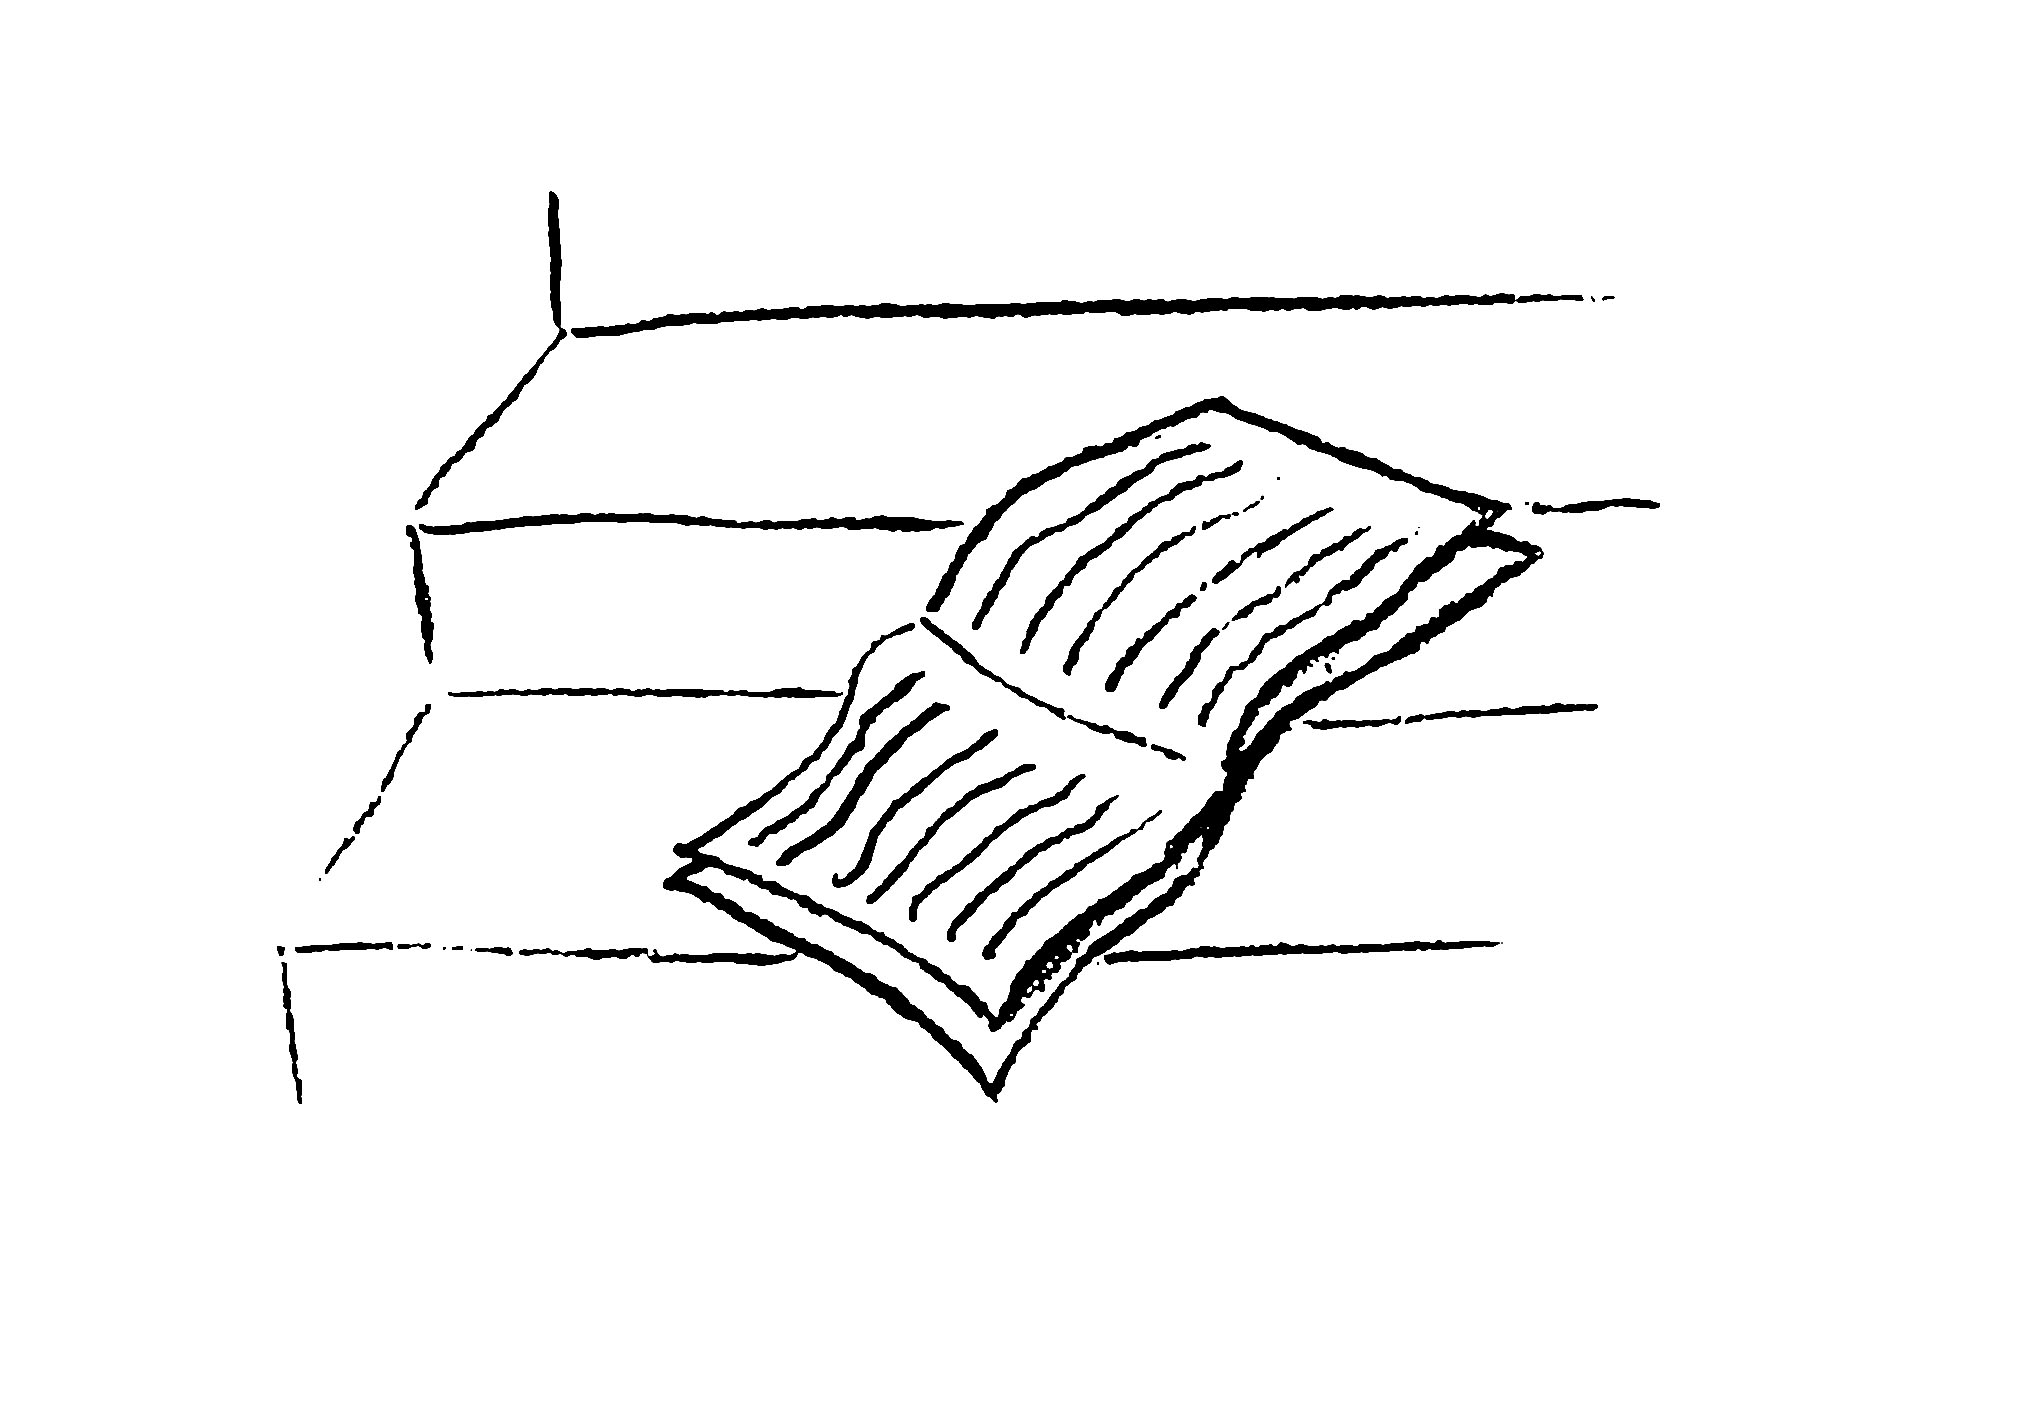
\includegraphics[width=0.95\columnwidth]{img/7.0 1 kniga.jpg}
\end{minipage}
\end{figure} 

\begin{thm}
    В блокноте 10 страниц, на каждой из них написано утверждение: 
    \par
    на первой странице: «В этом блокноте количество неверных утверждений делится на 1»;
    \par
    на второй странице: «В этом блокноте количество неверных утверждений делится на 2»;
    \par
    на третьей: «В этом блокноте количество неверных утверждений делится на 3»;
    \par
    ...
    \par
    на десятой: «В этом блокноте количество неверных утверждений делится на 10».
    \par
    Сколько в блокноте верных утверждений?
\end{thm}

\begin{thm}
    Чего больше: пятниц, кроме тех пятниц, которые не являются тринадцатыми числами, или тринадцатых чисел, кроме тех, которые не являются пятницами?
\end{thm}

\begin{thm}
    Предположим, что справедливы следующие утверждения:
    \par
    а) Среди людей, имеющих обезьянок, есть такие, которые не являются спелеологами.
    \par
    б) Люди, выращивающие кактусы, но не являющиеся спелеологами, не имеют обезьянок.
    \par
    Верно ли тогда, что не все владельцы обезьянок разводят кактусы?
\end{thm}

\begin{thm}
    Известно, что ляпусики, у которых есть варкала, не все бармаглоты. Кроме того, у тех ляпусиков, которые умеют хрюкотать и при этом не бармаглоты, варкал нет. Верно ли, что не все ляпусики, у которых есть варкала, умеют хрюкотать?
\end{thm}

\begin{thm} $^n$
    В тюрьму поместили 2011 узников. Надзиратель сказал им: «Я дам вам вечер поговорить друг с другом, а потом общаться вы не сможете. Иногда я буду одного из вас отводить в комнату, в которой есть лампа (вначале она выключена). Можно её включить или выключить. Если в какой-то момент кто-то из вас скажет мне, что вы все уже побывали в комнате, и будет прав, то я вас освобожу. А если неправ – казню. Если будете молчать, то все побываете в комнате, и ни для кого никакое посещение комнаты не станет последним». 
    \par
    Придумайте стратегию, гарантирующую узникам освобождение.
\end{thm}

\begin{figure}[H]
\begin{minipage}{0.69\linewidth}\setlength{\parindent}{1.5em}
    \begin{thm}
        Эрик увидел двух двухголовых дракончиков, головы которых спутались. Драконы бывают либо правдивые, т.е. все головы говорят только правду, либо лживые, т.е. все головы всегда лгут. Эрик решил помочь дракончикам распутать головы. Но для этого ему надо знать, где чья голова. Он спросил, какая голова чья у дракончиков, на что головы ответили: 
        \par первая голова: «я – правдивая голова»;
        \par вторая голова: «третья голова – моя родная голова»; 
        \par третья голова: «вторая голова – не родная мне голова»; 
        \par четвёртая голова: «третья голова – лживая». 
        \par Какие головы принадлежат каким дракончикам?
    \end{thm}
\end{minipage}
\hfill
\begin{minipage}{0.3\linewidth}
    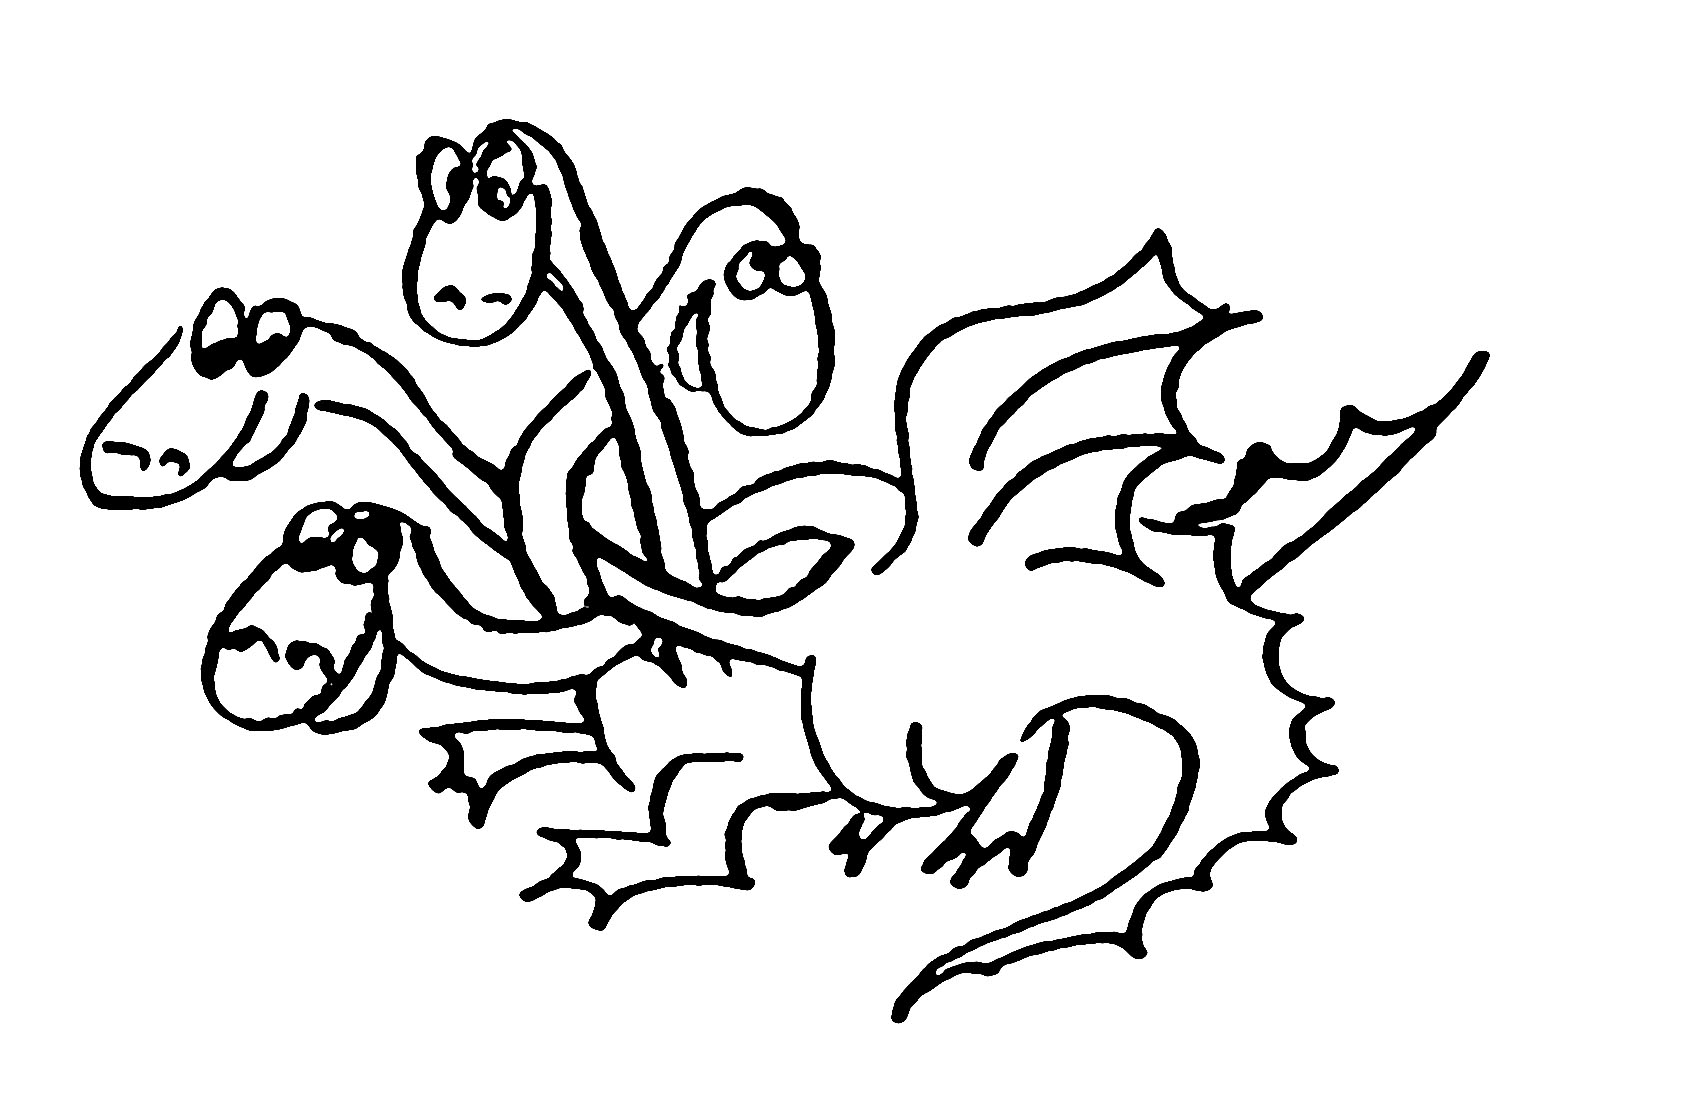
\includegraphics[width=0.95\columnwidth]{img/7.0 2 drakon.jpg}
\end{minipage}
\end{figure} 

\begin{thm} $^*$
    (по мотивам задачи Эйнштейна\footnotemark) В пяти домах с крышами разных цветов на одной стороне улицы живут пять джентльменов, каждый из которых предпочитает определённый напиток, занимается определённым видом спорта и держит животное, птицу, или разводит рыб (напитки, виды спорта и питомцы у всех разные). Известно, что:
    \par \textit{англичанин} живёт в доме с \textit{красной} крышей; 
    \par \textit{швед} держит \textit{собаку};
    \par \textit{датчанин} предпочитает \textit{чай}; 
    \par дом с \textit{зелёной} крышей расположен слева по соседству с домом под \textit{белой} крышей; 
    \par джентльмен из дома под \textit{оранжевой} крышей замечен за игрой в \textit{регби};
    \par \textit{футболист} иногда разговаривает с \textit{попугаем}; 
    \par хозяин дома с \textit{зелёной} крышей пьет \textit{кофе}, а хозяин \textit{среднего} дома – \textit{молоко};
    \par \textit{норвежец} живет в \textit{крайнем} доме, по соседству с домом с \textit{синей} крышей; 
    \par \textit{волейболист} соседствует с \textit{любителем коше}к; 
    \par \textit{любитель лошадей} живет рядом с \textit{регбистом}; 
    \par \textit{немец} играет в \textit{теннис}; 
    \par \textit{сосед волейболиста} пьет только \textit{минеральную воду}, а \textit{баскетболист} предпочитает \textit{квас}.
    \par Выясните, кто в каком доме живёт, каким видом спорта занимается, какие напитки предпочитает, а также кто разводит рыбок.
\end{thm}\footnotetext{Эйнштейн утверждал, что эту задачу не сможет решить более двух процентов мыслящего населения планеты. Интересно, к какой части относитесь вы?}

\section{Высказывания и отрицания.}

\begin{thm}
    Жители города Запузыринска ходят на руках и говорят все наоборот. Например, вместо «здравствуй» они говорят «до свидания», вместо «заходите в гости» – «катись отсюда», а вместо «вышел зайчик погулять» – «зашёл волчище посидеть». А вот какие задачи дают там на уроках математики: «Во вторую ночь заяц выплюнул 100 волков, а в первую – на 5 волков больше. Сколько волков выплюнул заяц в первую ночь?»
    \par
    а) Попробуйте перевести эту задачу на русский язык и дайте ответ.
    \par
    б) Переведите строчку из популярной запузыринской песни: “Огромной берёзе жарко летом”.
\end{thm}

\setlist{nosep} % Убирает вертикальные отступы между айтемами во всех листах


\begin{thm}
    «Все критяне – лжецы», – сказал философ с острова Крит. Какие из следующих утверждений верны, а какие нет, а о каких ничего нельзя сказать? Ответ обоснуйте.
    
    \begin{enumerate}[label=\asbuk*), ref=\asbuk*]
        \item Все критяне – лжецы.
        \item Все критяне говорят правду.
        \item Философ – лжец.
        \item Философ говорит правду.
        \item Среди критян есть лжецы.
        \item Среди критян есть говорящие правду.
    \end{enumerate}
    
\end{thm}


\begin{thm}
    Гоша \textit{верно} решил \textit{все} уравнения. Какие из перечисленных ниже утверждений являются отрицанием этого утверждения?
    
    \begin{enumerate}[label=\asbuk*), ref=\asbuk*]
        \item Петя решил верно все уравнения.
        \item Гоша решил неверно все уравнения.
        \item Гоша решил неверно одно уравнение.
        \item Гоша решил неверно какое-то уравнение.
        \item Гоша решил верно одно уравнение.
        \item Кто-то решил верно все уравнения
        \item Кто-то решил неверно все уравнения.
        \item Кто-то решил неверно какое-то уравнения.
    \end{enumerate}
    
\end{thm}


\begin{thm}
    На Уральском турнире матбоев в \textit{каждом} туре \textit{все} команды решили \textit{все} задачи. Какие из перечисленных ниже утверждений должны быть истинны\footnotemark, чтобы это утверждение стало неверным?
    
    \begin{enumerate}[label=\asbuk*), ref=\asbuk*]
        \item Была команда, которая в каждом туре не решила хотя бы одну задачу
        \item В каждом туре все команды не решили хотя бы одну задачу.
        \item Была команда, которая в каждом туре решила все задачи.
        \item Был тур, в котором ни одна из команд не решила все задачи.
        \item Была команда, которая в одном из туров решила все задачи.
        \item Во всём турнире была задача, которую не решила ни одна команда.
        \item В каждом туре все команды решили хотя бы одну задачу.
    \end{enumerate}
    
\end{thm}\footnotetext{Т.е. истинность этих утверждений является \textit{достаточной}, для того, чтобы сделать вывод.}


\begin{thm}
    На Уральском турнире матбоев \textit{не в каждом} туре \textit{все} команды решили \textit{все} задачи. Пусть это утверждение верно. Какие из перечисленных ниже утверждений обязательно должны быть истинны в этом случае?\footnotemark

    \begin{enumerate}[label=\asbuk*), ref=\asbuk*]
        \item Была команда, которая в каждом туре не решила хотя бы одну задачу
        \item В каждом туре все команды не решили хотя бы одну задачу.
        \item Была команда, которая в каждом туре решила все задачи.
        \item Был тур, в котором ни одна из команд не решила все задачи.
        \item Была команда, которая в одном из туров решила все задачи.
        \item Во всём турнире была задача, которую не решила ни одна команда.
        \item В каждом туре все команды решили хотя бы одну задачу.
    \end{enumerate}
\end{thm}\footnotetext{Т.е. истинность этих утверждений является \textit{необходимой}.}


\begin{thm}
    Назовём контрольную легкой, если за каждой партой найдется ученик, решивший все задачи. Дайте определение \textit{трудной} контрольной.
\end{thm}

\begin{thm}
    Рассмотрим два определения лёгкой контрольной: 
    \par 1) в каждом варианте каждую задачу решил хотя бы один ученик;
    \par 2) в каждом варианте хоты бы один ученик решил все задачи. 
    \par Может ли контрольная быть лёгкой в смысле определения 1) и трудной в смысле определения 2)?
\end{thm}


\section{Логические парадоксы.} 

Мы свободно говорим об истинности утверждений, высказываний... А что такое высказывание?
\par
Например, можно ли что-нибудь сказать об истинности или ложности следующих предложений:

\begin{center}
    \fbox{\begin{varwidth}{0.95\textwidth}
        Утверждение в рамке ложно
    \end{varwidth}}
\end{center}

\begin{center}
    \fbox{\begin{varwidth}{0.95\textwidth}
        \fbox{\begin{varwidth}{0.95\textwidth}
            Утверждение в двойной рамке истинно
        \end{varwidth}}
    \end{varwidth}}
\end{center}

\textit{Высказывание} – это утверждение, о котором можно сказать, истинно ли оно или ложно. Если
какое-то высказывание истинно, то его отрицание\footnote{Если рассматривать утверждения как все возможные события, то само утверждение – это множество некоторых событий, для которых это утверждение справедливо, а отрицание данного утверждения – все события, которые лежат вне этого множества.} ложно (обозначение: $A$ – само высказывание,
$\neg A$ – его отрицание). Понятно, что утверждение ''$A$ или $\neg A$ » всегда истинно (закон исключения третьего, другими словами, третьего не дано), напротив, утверждение ''$A$ и $\neg A$'' всегда ложно (закон противоречия), а двойное отрицание утверждения равносильно самому утверждению: $\neg \neg A = A$ (закон двойного отрицания).

В обычном языке можно придумать много предложений, о которых нельзя сказать, истинны они или ложны. Однако и в рамках логики существуют такие конструкции, о которых нельзя сказать, истинны они или ложны. Такие конструкции называются парадоксами. Например:

\begin{center}
    \begin{tabular}{ | m{6cm} | m{6cm} | } 
        \hline
        \textit{Утверждение справа истинно} & \textit{Утверждение слева ложно.} \\ 
        \hline
    \end{tabular}
\end{center}

\begin{figure}[H]
\begin{minipage}{0.79\linewidth}\setlength{\parindent}{1.5em}
    \begin{thm}
        \textit{(парадокс брадобрея)} Одному солдату отдали приказ брить тех и только тех, кто не бреется сам. Сможет ли он его выполнить?
    \end{thm}
    \begin{thm}
        Существует ли наименьшее целое число, которое нельзя определить при помощи фразы, состоящей не более чем из ста русских слов?
    \end{thm}
    \begin{thm}
        Как-то в 1943 году, шведское радио сообщило о том, что на следующей неделе намечено объявить воздушную учебную тревогу. Чтобы проверить готовность войск ПВО, учение решено провести внезапно так, что даже в день тревоги, ни один человек не сможет предугадать, в котором часу оно будет объявлено. Л. Экбом, преподаватель математики в Стокгольме, усмотрел в этом логический парадокс и обсудил его со своими студентами. Как вам кажется, в чём состоит этот парадокс?
    \end{thm}
\end{minipage}
\hfill
\begin{minipage}{0.2\linewidth}
    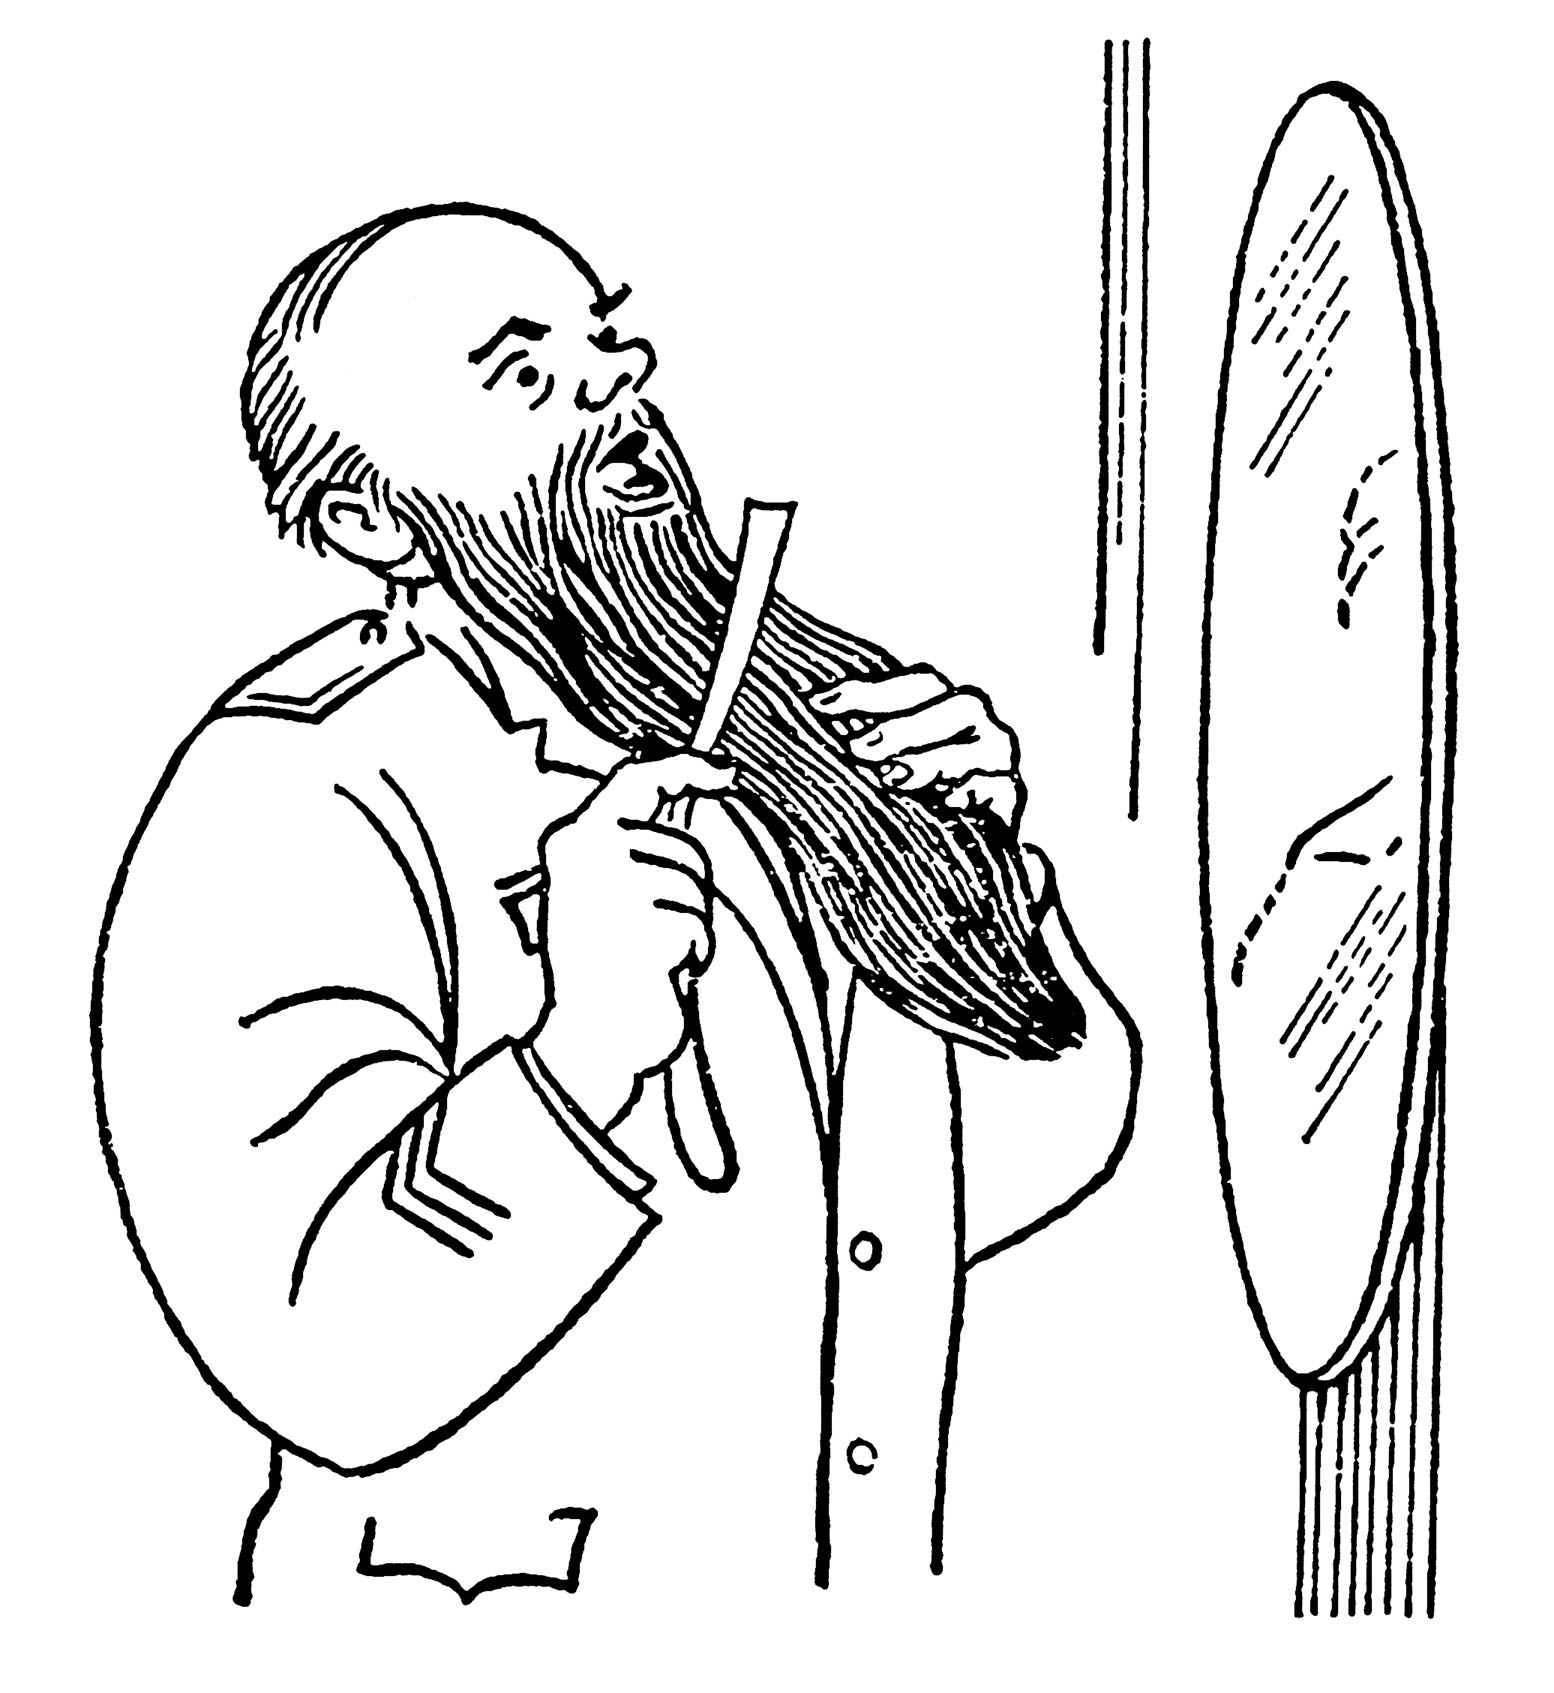
\includegraphics[width=0.95\columnwidth]{img/7.0 3 boroda.jpg}
\end{minipage}
\end{figure} 

\begin{thm}
    Племя людоедов поймало Робинзона Крузо. Вождь сказал: «Мы бы рады отпустить тебя, но по нашему закону ты сначала должен что-нибудь сказать. Если это окажется истиной – мы съедим тебя. Если же это будет ложью – тебя съест наш лев». Как спасти Робинзона?
\end{thm}

\section{Причина и следствие или «Если ... , то ... »}

\epigraph{\textit{«Если дважды два – пять, то существуют ведьмы...»}}{\textit{Феликс Хаусдорф}}

\begin{thm}
    За день до дождя Мюллер всегда чихает. Сегодня Мюллер чихнул. «Завтра будет дождь», – подумал Штирлиц. Прав ли он?
\end{thm}

\begin{figure}[H]
\begin{minipage}{0.79\linewidth}\setlength{\parindent}{1.5em}
    \begin{thm}
    Сформулируйте хотя бы одно
        \begin{enumerate}[label=\asbuk*), ref=\asbuk*]
        \item необходимое и достаточное;
        \item необходимое, но не достаточное;
        \item достаточное, но не необходимое;
        \item не необходимое и не достаточное
        \end{enumerate}
    условие того, что четырехугольник является трапецией.
    \end{thm}
\end{minipage}
\hfill
\begin{minipage}{0.2\linewidth}
    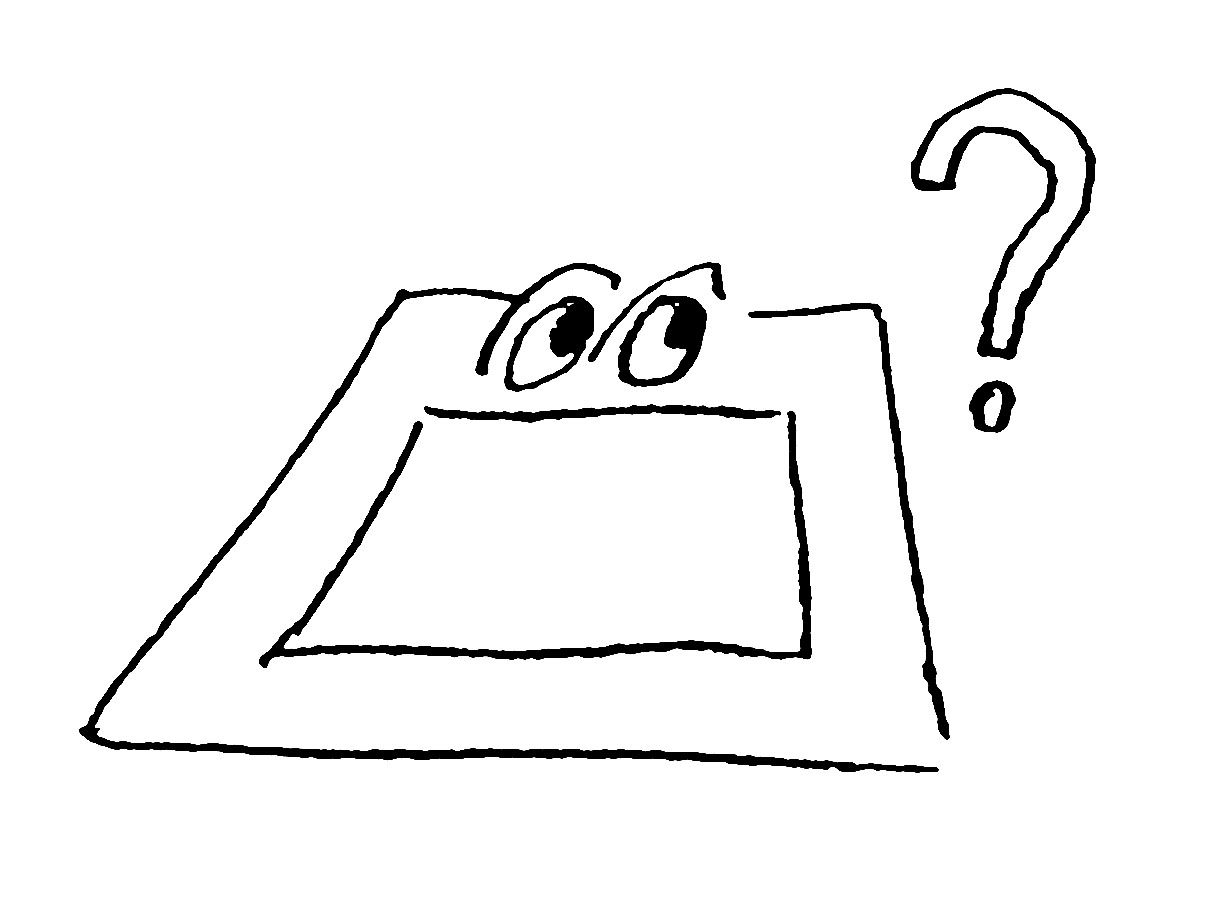
\includegraphics[width=0.95\columnwidth]{img/7.0 4 figura.jpg}
\end{minipage}
\end{figure} 

\begin{thm} \label{8.1 thm1}
    Пусть утверждение $B$: «Этот четырёхугольник – трапеция», а в качестве утверждения $A$ возьмём следующее: «У этого четырёхугольника есть две параллельные стороны». Сформулируйте 8 утверждений:
    \par
    1. Если $A$, то $B$. \hfill 2. Если $A$, то не $B$. \hfill 3. Если не $A$, то $B$. \hfill 4. Если не $A$, то не $B$.
    \par
    5. Если $B$, то $A$. \hfill 6. Если $B$, то не $A$. \hfill 7. Если не $B$, то $A$. \hfill 8. Если не $B$, то не $A$.
    \par
    Какие из этих утверждений верны, а какие нет?
\end{thm}

\begin{thm} \label{8.1 thm3}
    Пусть теперь $A$ и $B$ – какие-то утверждения (каждое из них либо истинно, либо ложно). Рассмотрим восемь теорем:
    \par
    1. Если $A$, то $B$. \hfill 2. Если $\overline{A}$, то $B$. \hfill 3. Если $A$, то $\overline{B}$. \hfill 4. Если $\overline{A}$, то $\overline{B}$.
    \par
    5. Если $B$, то $A$. \hfill 6. Если $\overline{B}$, то $A$. \hfill 7. Если $B$, то $\overline{A}$. \hfill 8. Если $\overline{B}$, то $\overline{A}$.
    \par
    Известно, что теорема 1 верна. Разбейте оставшиеся семь теорем на три группы: те, которые заведомо верны, те, которые заведомо неверны и те, о которых ничего определённо сказать нельзя (т.е. они могут быть верными или неверными в зависимости от выбора утверждений $A$ и $B$).\footnotemark
\end{thm}\footnotetext{Договоримся не рассматривать в качестве $A$ и $B$ утверждения, которые всегда истинны или всегда ложны, например, ''В квадрате все углы тупые'' или ''На плоскости прямые параллельны или пересекаются''.}

Заметим, что предыдущую задачу можно интерпретировать на языке множеств. Т.к. в высказывании речь идёт о некоторых объектах, то по отношению, скажем, к высказыванию $A$ все эти объекты можно разбить на два множества: множество объектов, для которых высказывание верно и множество, для которых неверно. Так сказать, $A$ и $\overline{A}$. (Например, утверждение $A$: «Данный четырёхугольник – параллелограмм», утверждение $B$: «данный четырёхугольник имеет равные стороны».) Тогда что на языке множеств означает наша теорема 1? Только то, что если объект принадлежит множеству $A$, то он принадлежит и множеству $B$!

\begin{thm} $^*$
    Какой смысл по-вашему мнению имеет высказывание Феликса Хаусдорфа, вынесенное в эпиграф?
\end{thm}

\begin{thm} \label{8.1 thm2}
    Однажды утром метеостанция маленького города Новозыбкова передала необычный прогноз погоды. Этот прогноз состоял из нескольких утверждений:
    \begin{enumerate}
        \item Если сегодня дождя не будет, то завтра будет ветреная погода.
        \item Если сегодня пойдёт дождь, то завтра без осадков.
        \item Если сегодня будет холодно, то влажность воздуха сегодня будет высокой.
        \item Если сегодня будет тепло, то завтра безветренно.
        \item Если сегодня ветра нет, то завтра будет тепло при высокой влажности и дождь.
        \item Если сегодня ветреная погода, то завтра – низкая влажность воздуха, но будет дождь.
        \item Если сегодня влажность будет высокой, то завтра она останется без изменений.  
    \end{enumerate}
    Допустим, что каждое утверждение синоптиков верно. Определите в этом случае погоду (т.е. температуру, осадки, влажность и ветер) на сегодня и завтра.
\end{thm}


\begin{center}
    \textit{\textbf{Лирическое отступление.}}
\end{center}

В курсе геометрии вы доказывали следующие утверждения: «Если четырёхугольник – параллелограмм, то его стороны попарно равны.», «Если четырёхугольник – параллелограмм, то его диагонали делятся точкой пересечения пополам.» Отсюда справедливо утверждение: «Если четырёхугольник – параллелограмм, то его стороны попарно равны и диагонали делятся точкой пересечения пополам».
Рассмотрим ещё один пример. В школьной столовой сок стоит 3 руб., а булочка – 2 руб. Справедливы следующие утверждения: «Если у Полины есть 3 рубля, то она может купить булочку.», «Если у Полины
есть 3 рубля, то она может купить сок.» Отсюда справедливо утверждение: «Если у Полины есть 3 рубля, то
она может купить булочку и сок.» ... Рассуждения аналогичны. В чём тут дело?

\section{«Сложносочинённые» утверждения.}

Пусть имеется набор некоторых высказываний, про которые можно узнать, истинны они или ложны. Будем обозначать их заглавными буквами: $A$, $B$, $C$ и т.д. Как и в обычном языке, из уже имеющихся высказываний можно, как из кирпичиков, строить новые. Например, в задачах \ref{8.1 thm1} – \ref{8.1 thm2} высказывания были построены с помощью конструкции «если $A$, то $B$»\footnote{В этом случае высказывание $A$ называется посылкой, а высказывание $B$ – следствием или заключением}. Как из простых предложений можно строить сложносочинённые предложения, где все входящие предложения равноправны, так и из «простых» высказываний можно строить сложные с помощью союзов «и» и «или».

\begin{dfn}
    Пусть $A$ и $B$ – некоторые высказывания. Тогда $A \vee B$ – \textit{дизъюнкция (логическое сложение)} высказываний $A$ и $B$. (Читается «$A$ или $B$» ) Это высказывание истинно, когда хотя бы одно из входящих в него простых высказываний истинно, а ложно, когда ложны все высказывания.
\end{dfn}

\begin{dfn}
    Аналогично, $А \& \ В$\footnote{Также используется обозначение $A \wedge B$.} – \textit{конъюнкция (логическое умножение)} высказываний $A$ и $B$. (Читается «$A$ и $B$» ) Это высказывание истинно только когда истинны все входящие в него высказывания, а ложно, когда ложно хотя бы одно.
\end{dfn}

Для наглядности запишем в табличку:

\begin{figure}[H]
\begin{minipage}{0.45\linewidth}\setlength{\parindent}{1.5em}
    \begin{center}
        \begin{tabular}{ |c|c|c| } 
            \hline
             $A$ & $B$ & $A \vee B$ \\ 
             \hline
             \textit{истина} & \textit{истина} & \textit{истина} \\ 
             \hline
             \textit{истина} & \textit{ложь} & \textit{истина} \\ 
             \hline 
             \textit{ложь} & \textit{истина} & \textit{истина} \\ 
             \hline 
             \textit{ложь} & \textit{ложь} & \textit{ложь} \\ 
             \hline
        \end{tabular}
    \end{center}
\end{minipage}
\hfill
\begin{minipage}{0.45\linewidth}
    \begin{center}
        \begin{tabular}{ |c|c|c| } 
            \hline
             $A$ & $B$ & $A\  \& \ B$ \\ 
             \hline
             \textit{истина} & \textit{истина} & \textit{истина} \\ 
             \hline
             \textit{истина} & \textit{ложь} & \textit{ложь} \\ 
             \hline 
             \textit{ложь} & \textit{истина} & \textit{ложь} \\ 
             \hline 
             \textit{ложь} & \textit{ложь} & \textit{ложь} \\ 
             \hline
        \end{tabular}
    \end{center}
\end{minipage}
\end{figure} 

Почему эти операции называют сложением и умножением станет понятнее, если считать значение «истина» равным 1, а значение «ложь» – 0.\footnote{Правда, при сложении нам придется договориться, что 1 + 1 = 1.}

\begin{ex}
    Решите примеры:
    \par
    \textbf{1}. 1 $\vee$ 0 = ? \hfill 
    \textbf{2}. 0 $\&$ 1 = ? \hfill
    \textbf{3}. 1 $\&$ (0 $\vee$ 1) = ? \hfill
    \textbf{4}. (1 $\&$ 1) $\vee$ (0 $\vee$ 1) = ? \hfill
    \textbf{5}. 0 $\vee$ (0 $\vee$ (0 $\vee$ 1)) = ?
\end{ex}

\begin{ex}
    Вычислите значение выражения, если $A$ истинно, а $B$ - ложно:
    \par
    \textbf{1}. $B$ $\vee$ $A$ \hfill 
    \textbf{2}. $A$ $\&$ $\overline{B}$ \hfill
    \textbf{3}. $A$ $\&$ ($\overline{A}$ $\vee$ $\overline{B}$) = ? \hfill
    \textbf{4}. ($\overline{A}$ $\&$ $\overline{B}$) $\vee$ ($\overline{A}$ $\vee$ $B$) \hfill
    \textbf{5}. $\overline{A}$ $\vee$ ($\overline{B}$ $\vee$ ($B$ $\vee$ $A$))
\end{ex}

\begin{thm}
    Антон лжёт по понедельникам, вторникам и средам, а в остальные дни говорит только правду. Выясните, в какие дни недели Антон может заявить:
    \par а) Я лгал вчера и буду лгать завтра.
    \par б) Я лгал вчера или буду лгать завтра. 
    \par в) Я не лгал вчера и не буду лгать завтра.
    \par г) Я не лгал вчера или не буду лгать завтра.
\end{thm}

\begin{thm}
    Известно, что утверждение «$A$ или не $B$» истинно. Что вы можете сказать про истинность утверждений $A$ и $B$. А если утверждение «$A$ или не $B$» ложно?
\end{thm}

\begin{thm}
    На улице \textit{светит солнце} и у Оли \textit{плохое} настроение. Какие из перечисленных ниже утверждений являются отрицанием этого утверждения?
    \begin{enumerate}[label=\asbuk*), ref=\asbuk*]
        \item На улице пасмурно и у Оли хорошее настроение.
        \item На улице пасмурно или у Оли хорошее настроение.
        \item На улице пасмурно и у Оли плохое настроение.
        \item На улице пасмурно или у Оли плохое настроение.
        \item На улице светит солнце и у Оли хорошее настроение.
        \item На улице светит солнце или у Оли хорошее настроение.
    \end{enumerate}
\end{thm}

\begin{thm}
    На уроке алгебры Андрей получил \textit{пятёрку или четвёрку}. Какие из перечисленных ниже утверждений являются отрицанием этого утверждения?
    \begin{enumerate}[label=\asbuk*), ref=\asbuk*]
        \item На уроке алгебры Андрей получил пятёрку и четвёрку.
        \item На уроке алгебры Андрей получил двойку и тройку.
        \item На уроке алгебры Андрей получил двойку или тройку.
        \item На уроке алгебры Андрей не получил пятёрку и не получил четвёрку.
        \item На уроке алгебры Андрей не получил пятёрку или не получил четвёрку.
        \item На уроке алгебры Андрей получил пятёрку, но не получил четвёрку.
        \item На уроке алгебры Андрей не получил пятёрку, но получил четвёрку.
    \end{enumerate}
\end{thm}

\begin{dfn}
    Пусть $А$ и $В$ – некоторые высказывания. Конструкция «если ... , то ... » называется \textit{логическим следованием} или \textit{импликацией}. Обозначение $А \Rightarrow В$.
\end{dfn}

\begin{ex}
    Составьте табличку значений для импликации и сравните полученные результаты с результатом задачи \ref{8.1 thm3}.
\end{ex}
\head{Сентябрь}{Листок 8. Логика. Уровень 0.}

\epigraph{\textit{– Разве это ложь? – сказала Королева. – Слыхала я такую
ложь, рядом с которой эта правдива, как толковый словарь!}}{\textit{Л. Кэрролл "Алиса в Зазеркалье"}}

Безусловно, вы уже сталкивались с задачами, в которых нужно рассматривать случай, когда кто-то лжёт. Соответственно встаёт вопрос об истинности или ложности некоторых утверждений. Позже мы разберём это подробнее, а пока то, что есть «правда», а что «ложь», мы будем считать интуитивно понятным. Для начала несколько простых упражнений.
\\
Напомним, что «рыцари» всегда говорят правду, а «лжецы» всегда лгут.

\begin{ex}
    Известно, что в ящике лежит 17 шариков. Какие из приведенных ниже утверждений являются всегда истинными, а какие – всегда ложными
    \begin{enumerate}[label=\asbuk*), ref=\asbuk*]
        \item В ящике не менее 17 шариков.
        \item В ящике лежит 17 шариков или 15 шариков.
        \item В ящике найдётся 15 шариков.
        \item В ящике есть шарики разных цветов.
        \item В ящике найдётся не более 17 одноцветных шариков.
        \item В ящике не менее двух шариков одного размера.
        \item Из ящика нельзя вытащить 20 шариков одного цвета.
        \item Шарики в ящике можно сложить по парам.
    \end{enumerate}
\end{ex}

\begin{ex}
    После победы над Змеем Горынычем три богатыря заявили:
    \par
    \underline{Илья Муромец}: «Змея убил Добрыня Никитич».
    \par
    \underline{Добрыня Никитич}: «Змея убил Алёша Попович».
    \par
    \underline{Алёша Попович}: «Змея убил я».
    \par
    Кто убил Змея и почему именно он, если только один из них сказал правду?
\end{ex}

\begin{ex}
    В комнате находятся рыцарь и лжец. Кто из них мог сказать фразу: «Мы оба лжецы»?
\end{ex}

\begin{ex}
    На острове рыцарей и лжецов житель $A$ в присутствии другого жителя $B$ говорит: «По крайней мере один из нас – лжец». Кто такие $A$ и $B$?
\end{ex}

\begin{ex}
    В комнате 2012 жителей острова рыцарей и лжецов. Каждый из них заявил: «Кроме меня в комнате все лжецы!». Сколько рыцарей в комнате?
\end{ex}

\begin{ex}
    В комнате 2012 жителей острова рыцарей и лжецов. Одного из них зовут Ваня. Они встали в круг, и Миша – правый сосед Вани – сказал: «Ваня, ты лжец!». Тогда правый сосед Миши сказал: «Ты не прав!», и так далее: каждый (кроме Вани) по кругу высказал своему соседу, что он неправ. Сколько в комнате лжецов?
\end{ex}

\begin{ex}
    А если в предыдущей задаче каждый (кроме Вани) сказал «Ты прав!», то сколько тогда было бы в комнате лжецов?
\end{ex}

\begin{ex}
    У Снусмумрика украли флейту. Известно, что те, кто крадут флейты, всегда лгут. «Я знаю, кто украл флейту!», – заявил Мумми-тролль. Виновен ли Мумми-тролль?
\end{ex}

\begin{ex}
    Среди трёх человек $A$, $B$ и $C$ один лжец, один рыцарь, а третий – нормальный человек, который может говорить и правду, и ложь. 
    $A$ говорит: «Я нормальный человек».
    $B$ говорит: «$A$ и $C$ иногда говорят правду». 
    $C$ говорит: «$B$ – нормальный человек».
    Кто из них кто?
\end{ex}

\begin{ex}
     В конференции участвовало 100 человек – химиков и алхимиков. Каждому был задан вопрос: «Если не считать Вас, то кого больше среди остальных участников – химиков или алхимиков?». Когда опросили 51 участника, и все ответили, что алхимиков больше, опрос прервался. Алхимики всегда лгут, а химики говорят правду. Сколько химиков среди участников?
\end{ex}

\begin{ex}
    В комнате четыре человека – жители острова рыцарей и лжецов каждый из них сделал заявление.
    \par
    Первый: «среди нас не более одного лжеца».
    \par
    Второй: «среди нас не более двух лжецов».
    \par
    Третий: «среди нас не более трех лжецов».
    \par
    Четвёртый: «среди нас не более четырех лжецов».
    \\
    Сколько рыцарей в комнате?
\end{ex}

\begin{ex}
    У Карабаса-Барабаса украли пять золотых. Карабас подозревает в краже лису Алису, кота Базилио, Дуремара и Буратино, так как неопровержимыми уликами установлено, что 
    \par
    кто-то из них обязательно виновен; 
    \par
    никто больше не мог это сделать;
    \par
    Алиса всегда действует заодно с Базилио;
    \par
    если Дуремар виновен, то у него было ровно 2 соучастника;
    \par
    если Буратино виновен, то у него был ровно 1 соучастник.
    \\
    Нужно определить, виновен ли Базилио.
\end{ex}

\section{Наконец-то, задачи!}

В следующих задачах не требуется ничего, кроме здравых рассуждений. Напоминаем, что задачи, отмеченные значком \textit{п}, являются письменными, и в устном виде приниматься не будут. Отмеченные звёздочками не являются обязательными (это не значит, что они сложнее).

\begin{thm} $^n$
    Мама пришла с работы домой и обнаружила, что коробка с конфетами пуста. На вопрос «Кто съел конфеты?» её дочери Вета, Рая и Соня ответили так:
    \par
    Вета: «Соня не ела последнюю конфету» 
    \par
    Рая: «Соня и Вета обе ели конфеты»
    \par 
    Соня: «Рая и Вета обе не ели конфеты».
    \\ 
    Впоследствии оказалось, что все сказали неправду. Кто съел конфеты?
\end{thm}

\begin{thm}
    На острове невезения живут 2012 человек. Некоторые из них всегда лгут, а остальные всегда говорят правду. Каждому жителю острова не везёт только в один из трёх дней: понедельник, среду или пятницу. Однажды каждому жителю острова задали три вопроса:
    \par
    1. «Вам не везёт в понедельник?»
    \par 
    2. «Вам не везёт в среду?»
    \par
    3. «Вам не везёт в пятницу?»
    \\
    На первый вопрос ответили «да» 999 человек, на второй – 1000, на третий – 1001. Сколько лжецов на острове?
\end{thm}

\begin{thm}
    В комнате сидело 2012 жителей острова рыцарей и лжецов. В какой-то момент один человек обиделся и ушёл. Один из оставшихся, поглядев в след, заметил: «Ушедший – лжец!» После чего встал и тоже вышел. Второй сказал: «Оба ушедшие – лжецы» и тоже ушёл. Далее каждый из оставшихся уходил, говоря: «Все ушедшие – лжецы». Пока последний оставшийся в комнате печально не констатировал: «Да, все ушедшие – лжецы».
    \\
    Определите, сколько в комнате было лжецов первоначально. (Лжецы всегда лгут, рыцари всегда говорят правду)
\end{thm}

\begin{thm}
    На планете «Куб» (имеющей форму куба) каждой гранью владеет рыцарь или лжец. Каждый из них утверждает, что среди его соседей лжецов больше, чем рыцарей. Сколько рыцарей и сколько лжецов владеют гранями планеты?
\end{thm}

\begin{thm}
    Однажды каждый житель планеты «Куб» из предыдущей задачи (возможно, теперь они владеют гранями планеты как--то по--другому) сделал заявление: «Среди моих соседей лжецов больше, чем рыцарей». Можно ли поменять местами двух человек, чтобы каждый из них мог сказать «Среди моих соседей рыцарей больше, чем лжецов»?
\end{thm}

\newpage

\begin{thm}
    Министры иностранных дел Ассирии, Аримака и Такито обсудили за закрытыми дверями проекты соглашения о полном разоружении, представленные каждой из стран. Отвечая затем на вопрос журналистов: «Чей именно проект был принят?», министры дали такие ответы:
    \par
    Ассирия: «Проект не наш. Проект не Аримаки»;
    \par
    Аримака: «Проект не Ассирии. Проект Такито»;
    \par
    Такито: «Проект не наш. Проект Ассирии».
    \\
    Один из них (самый откровенный) оба раза говорил правду; второй (самый скрытный) оба раза говорил неправду, третий (осторожный) один раз сказал правду, а другой раз – неправду. Определите, чей проект был принят.
\end{thm}

\begin{thm}
    а) Обязательно ли является ли старейший шахматист среди музыкантов старейшим музыкантом среди шахматистов?
    \par
    б) Обязательно ли является ли лучший шахматист среди музыкантов лучшим музыкантом среди шахматистов?\footnotemark
\end{thm}\footnotetext{Подумайте сначала, чем отличается шахматист среди музыкантов от музыканта среди шахматистов.}
\head{Сентябрь}{Листок 8. Логика. Уровень 1.}

% Уровень 1

\begin{thm}
    Школьники Иванов, Петров и Никитин сидели на скамейке. Их звали Ваня, Петя и Никита. Неожиданно Никитин сказал Пете: «А ты знаешь, что среди нас нет человека, у которого фамилия образована от его имени?» Назовите полные имена мальчиков. Под полным именем мальчика будем подразумевать его имя и фамилию.
\end{thm}

\begin{thm}
    Вася, Коля, Илья и Женя живут в разных городах: Москве, Киеве, Париже и Берлине. Известно, что если Женя живёт в Москве, то Илья не парижанин. Если же Илья – москвич, то Вася живёт не в Париже. Кроме того, известно, что Вася никогда не был в Москве и Киеве, а Коля – в Берлине и Париже. Илье не довелось побывать в Киеве и Берлине. А Женя мечтает съездить в Париж. В каких городах живёт каждый из мальчиков?
\end{thm}

\begin{thm}
    Костя, Женя и Миша имеют фамилии: Орлов, Соколов и Ястребов. Какую фамилию имеет каждый мальчик, если Женя, Миша и Соколов – члены математического кружка, а Миша и Ястребов занимаются музыкой?
\end{thm}

\begin{thm}
    3 мальчика, приехавшие в выездную школу из разных городов, рассказывают о себе:
    \par
    Петя: «Я живу в Москве, а Миша в Волгограде».
    \par
    Миша: «Я живу в Москве, а Петя в Архангельске».
    \par
    Коля: «Я живу в Москве, а Петя в Волгограде».
    \\
    Их учитель, удивлённый противоречиями в сказанном, попросил их объяснить, где правда, а где ложь. Тогда ребята признались, что в сказанном каждым из них одно утверждение – правда, а второе – ложно. В каком городе живёт каждый из мальчиков?
\end{thm}

\begin{thm} $^n$
    Ниф-Ниф, Наф-Наф и Нуф-Нуф пришли в казино в серебряной, золотой и платиновой цепях. Перстни у них были из тех же металлов. У Ниф-Нифа цепь и перстень были изготовлены из одинакового металла. У Наф-Нафа ни цепь, ни перстень не были серебряными. У Нуф-Нуфа цепь была из платины, а перстень не из платины. У кого из чего были изготовлены украшения?
\end{thm}

\begin{thm}
    Три друга – Пётр, Роман и Сергей – учатся на математическом, физическом и химическом факультетах. Если Пётр – математик, то Сергей не физик. Если Роман не физик, то Пётр - математик. Если Сергей не математик, то Роман – химик. Сможете ли Вы определить специальность каждого?
\end{thm}

\begin{thm}
    Дима, Катя, Миша, Света и Юра проводили лето на даче вместе с родителями. Все дети разного возраста: от 4-x до 8-ми лет. У каждого из них своя любимая еда (бананы, мороженое, пиццa, спагетти, шоколад). И каждый чего-нибудь боится (грозы, пауков, привидений, собак, темноты). Определите сколько лет каждому из них, у кого какая любимая еда, и кто чего боится.

    \begin{enumerate}
        \item Девочки старше остальных, ни одна из них не боится темноты, и обе не любят шоколад.
        \item Света обожает пиццу и не страшится пауков
        \item Пятилетний ребёнок больше всего боится привидений.
        \item Шестилетний ребёнок боится грозы и равнодушен к шоколаду и спагетти.
        \item Самый младший ребёнок любит есть бананы, а самый старший не боится собак.
        \item Ни Дима (ему не пять лет), ни Миша не боятся ни темноты, ни пауков, и оба не любят бананы.
    \end{enumerate}
    \textit{\textbf{Замечание.}} Считается, что возраст выражается целым числом лет без учёта месяцев.
\end{thm}

\begin{thm}
    Четыре подруги пришли на каток, каждая со своим братом. Они разбились на пары и начали кататься. Оказалось, что в каждой паре «кавалер» выше «дамы», и никто не катается со своей сестрой. Самым высоким в компании был Паша Воробьев, следующим по росту – Юра Егоров, потом – Люся Егорова, Серёжа Петров, Оля Петрова, Дима Крымов, Инна Крымова и Аня Воробьева. Кто с кем катался?
\end{thm}

\newpage

\begin{thm}
    В одном из институтов учатся 4 друга. Самый младший учится на 1 курсе, а старший – на 4. Известно, что Борис – персональный стипендиат, Василий летом должен ехать на практику в Омск, а Иванов – домой в Донбасс. Николай курсом старше Петра, Борис и Орлов – коренные ленинградцы, Крылов в прошлом учебном году окончил школу и поступил на факультет, где учится Карпов. Борис иногда пользуется прошлогодними конспектами Василия. Надо определить имя и фамилию каждого из друзей и курс, на котором он учится.
    \\
    \textit{\textbf{Замечание.}} Чтобы получить персональную стипендию нужно отучиться в институте не менее года.
\end{thm}

% Некоторые задачи вырезаны из-за того, что они уже есть в Оверлифе, в файле 8.0

% Уровень 1а

\begin{thm}
    Однажды в летнем лагере за круглым столом собрались пять ребят родом из Москвы, Астрахани, Новгорода, Перми, Костромы. Их звали: Юра, Толя, Лёша, Коля, Витя. Москвич сидел между Витей и жителем Костромы, астраханец – между Юрой и Толей, а напротив его сидели пермяк и Лёша. Коля никогда до этого не был в Астрахани, Юра не был в Москве и Костроме, а костромич с Толей регулярно переписываются. Определите, в каком городе живёт каждый из ребят.
\end{thm}

\begin{thm}
    За столиком в кафе собрались трое друзей: Белокуров, Рыжов и Чернов. Брюнет сказал Белокурову: «Любопытно, что один из нас блондин, другой брюнет, а третий рыжий, но ни у кого цвет волос не совпадает с фамилией». Какой цвет волос у каждого из них?
\end{thm}

% Файл "Уровень 2" состоит из второй половины Оверлифного файла 8.0. Как итог я добавил единственную не дублированную задачу из 2 Уровня сюда.

\begin{center}
    \textbf{«Перевёртыши»}
\end{center}
В выездных школах достаточно популярна игра в перевёртыши – когда известная фраза зашифровывается путём замены каждого из слов на условно противоположное. Например: По морю ёлка плыла (Во поле берёза стояла). Вам предлагается расшифровать приведённые ниже перевёртыши.
\begin{enumerate}
    \item Быстро сутки тонут близко. 
    \item Год помирай, год тупи.
    \item Некоторые жертвы могут догадаться, откуда прыгают ёжики.
    \item От одной лисы побежишь – всех разгонишь. 
    \item Десять на машине, включая кошку.
    \item Вы читали, вы читали, ваши ноженьки взбодрились.
    \item Птичка в небе полетала и сто баксов потеряла. Села птичка на забор – продавала всем топор.
    \item Один, один, один зелёный папоротник. 
    \item Три начала, три квадрата, и в конце гайка.
    \item Стоит Скиф около моря. Слышит Скиф – на море лебедь.
    \item Сиди тут – известно где, убери это – известно кого.
    \item Ежедневно знойным мигом ты в долину убегаешь.
    \item Стоит лягушка замирает, смеётся в остановке.
    \item Сдохли у ребёнка три занудных львёнка.
    \item Жара без мглы – поганый вечер.
    \item Подобрали зайку с крыши, прикрепили зайке крылья.
    \item У лисы какой-то чёрт отнял буханку хлеба.
\end{enumerate}
\head{Сентябрь}{Листок 8. Логика. Математический бой.}

\begin{enumerate}

    \item 
    Каждый житель острова Невезения — либо рыцарь, который всегда говорит правду, либо лжец, который всегда лжёт, причём лжецов на острове ровно 33. Однажды каждый житель острова заявил: «Среди всех жителей острова, не считая меня, не меньше трети лжецов». Сколько жителей может быть на острове? Перечислите все возможности и докажите, что других возможностей нет.
    
    \item 
    На собрании лжецов и рыцарей путешественник пытается определить самого старшего. Ему известно, что среди присутствующих лжецов и рыцарей поровну, а также, что возрасты всех различны. Ему разрешается выбрать любую группу людей и спросить любого из присутствующих, кто в этой группе самый старший. Докажите, что путешественник не сможет гарантированно определить самого старшего, сколько бы вопросов он ни задавал.
    
    \item 
    Рыцари и лжецы встали в хоровод, при этом некоторые из них знакомы, а некоторые -- нет. Каждый сказал своему левому соседу: «Я знаю, кто ты, и я знаю, что ты лжец». Докажите, что лжецов в круге не меньше половины.
    
    \item 
    Каждый островитянин произнёс две фразы: «Среди моих знакомых островитян более двух лжецов» и «Среди моих знакомых островитян более трёх рыцарей». Докажите, что лжецов на острове не меньше, чем рыцарей

    \item 
    На острове Невезения ровно 1 житель сказал: «Есть лжец выше меня», 
    \\ ровно 2 жителя сказали: «Есть хотя бы двое лжецов выше меня», 
    \\ ... , 
    \\ ровно 20 жителей сказали: «Есть хотя бы 20 лжецов выше меня». 
    \par Известно, что все островитяне — разного роста, и каждый житель высказался ровно один раз. Сколько лжецов живёт на острове? Напомним, что рыцари всегда говорят правду, а лжецы всегда лгут.

    \item 
    Среди 300 человек есть 100 Петь, 100 Гош и 100 Мить. После того, как каждому задали вопрос, как его зовут, получилось 100 ответов «Петя», 100 ответов «Гоша» и 100 ответов «Митя». Известно, что ровно 80 Петь и ровно половина Гош всегда лгут, а остальные Пети и Гоши всегда говорят правду. Какое наибольшее число Мить могут быть кристально честными?

    \item 
    На острове живут рыцари, которые всегда говорят правду и лжецы, которые всегда лгут. Встретились три островитянина: Михаил Михайлович, Сергей Сергеевич, и Анатолий Анатольевич. Михаил сказал: «Мы все лжецы». Сергей на это ему ответил: «Нет, только ты». Кто есть Анатолий  — рыцарь, или лжец?

    \item 
    На острове появилось новое сообщество -- хитрецы, которые иногда говорят правду, а иногда лгут. За круглым столом сидят представители рыцарей, лжецов, и хитрецов. Каждый из сидящих произнёс две фразы:
    \par 1) «Слева от меня сидит лжец.» 
    \par 2) «Справа от меня сидит хитрец.»
    \\ Докажите, что за этим столом рыцарей сидит столько же, сколько и лжецов.
    
    \item 
    Дорогу разделили на 2011 частей (не обязательно одинаковой длины). Яна знает длину дороги. Ей разрешено спросить, чему равно расстояние между серединами любых двух частей, при этом количество вопросов не ограничено. Длину каких частей она сможет узнать?

    \item 
    \textit{Лесногородская головоломка}. 
    \par Все жители санатория «Лесной Городок» делятся на 4 типа:
    \\ 1) Титаны в здравом уме; 
    \\ 2) Титаны, лишившиеся рассудка;
    \\ 3) Друиды, находящиеся в здравом уме
    \\ 4) Друиды, лишённые рассудка. 
    \\ Титаны в здравом уме всегда говорят истину (их утверждения правильны и сами титаны честны). Титаны, лишённые рассудка, всегда лгут (в силу собственных заблуждений, но не умышленно!). Друиды в здравом уме тоже всегда лгут (в силу своей природы, а не по заблуждению). 
    \\ Друиды, лишённые рассудка, всегда говорят правду (они убеждены в своих ложных утверждениях, но при этом умышленно лгут).
    \\ Однажды три Титана делились впечатлениями о прогулках по санаторию, совершенными в разное время. Первый Титан сказал:
    \\ -- Я встретил одного человека по имени Лёша и спросил его, является ли он Титаном в здравом уме. Он мне ответил вполне определённо («да» или «нет»), но я так и не понял, к какому типу он принадлежит.
    \\ -- Я тоже встретил этого Лёшу, -- сказал второй Титан. -- Я спросил у него, является ли он Друидом, лишившимся рассудка, и он ответил определённо («да» или «нет»), однако я не понял, кем он был в действительности.
    \\ -- Я тоже встретил этого Лёшу! -- воскликнул третий Титан. -- Я спросил у него, является ли он Друидом в здравом уме, и он также ответил определённо («да» или «нет»), однако я всё равно не понял, кто он!
    \\ Кто же такой -- Лёша?
\end{enumerate}
\chapter{Комбинаторика -- 2}
\head{Октябрь}{Листок 9. Комбинаторика -- 2. Уровень 1.}

\epigraph{\textit{Как-то у Насреддина спросили, сколько на небе звёзд. Он ответил:
\\
— Этот вопрос меня интересует с давних пор. Но я думаю, что решить его можно только в том случае, если самому подняться на небо и сосчитать звёзды. Однако тут возникают два препятствия: если начать эту работу днём, то боюсь, что множество дел и толпы зевак помешают мне. Остаётся только подняться ночью на небо и заняться подсчётом звезд. Но это тоже опасно, потому что я не знаю, смогу ли найти на небе свечи или лампу, а в ночной темноте подсчитывать звёзды невозможно. Вот эти два препятствия и мешают мне решить вопрос о количестве звёзд на небе.}}{\textit{«Притчи о Насреддине»}}

В прошлом году мы занимались подсчётом различных вариантов выполнить что-либо. Например, мы выясняли, сколькими способами можно расставить в ряд $k$ из $n$ предметов. В литературе одна такая выборка называется \textit{размещением} и обозначается $A^k_n$. Если мы выбираем все предметы, то получаем перестановку. Число перестановок обозначается $A_n$ или $P_n$. Мы доказывали, что $P_n = n$! Когда мы говорим о размещениях, то для нас имеет значение порядок, в котором мы выбираем предметы. Если же требуется выяснить лишь сколько различных наборов из $k$ элементов можно выбрать из данного множества, то любой такой набор называется сочетанием, а число сочетаний, т.е. количество различных наборов из $k$ элементов, которые можно выбрать из имеющихся $n$, обозначается $C^n_k$. 
\\
В частности справедлива формула \boxed{P_k \cdot C^k_n = A^k_n}

\section{Посчитаем варианты, или «шары и перегородки».}

\epigraph{\textit{-- Чем займёмся, уважаемые кроты?
\\
-- А почему бы нам не посчитать?}}{\textit{Из мультфильма «Дюймовочка»}}

\begin{figure}[H]
\begin{minipage}{0.75\linewidth}\setlength{\parindent}{1.5em}
    \begin{thm}
        Сколькими способами можно разбить наш класс на две (необязательно равные) команды?
    \end{thm}
    \begin{thm}
        У Эрика есть 20 друзей и каждый день он приглашает некоторых из них в гости так, чтобы компания ни разу не повторялась (в какой-то день он может не пригласить никого). Сколько дней он сможет так делать?
    \end{thm}
    \begin{ques}
        Что общего между двумя предыдущими задачами?
    \end{ques}
\end{minipage}
\hfill
\begin{minipage}{0.2\linewidth}
    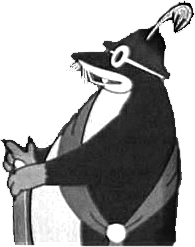
\includegraphics[width=0.95\columnwidth]{img/9.0.1 krot.png}
\end{minipage}
\end{figure} 

\begin{thm}
    Сколькими способами можно разложить 2009 конфет в 17 коробок так, чтобы в каждой коробке была хотя бы одна конфета? (Конфеты считать одинаковыми, коробки разными)
    \par
    \textit{\textbf{Ответ.}} $C^{16}_{2008} = \dfrac{2008 \cdot 2007 \cdot ... \cdot 1993}{16!}$
    \par
    \textit{\textbf{Решение.}} Разложим все 2009 конфет в ряд и будем расставлять между ними перегородки. Поскольку коробок 17, то перегородок потребуется 16. Все, что будет ДО первой перегородки, положим в первую коробку, от 1 до 2 – во вторую коробку, от 2 до 3 – в третью и так далее, всё, что ПОСЛЕ шестнадцатой перегородки – положим в семнадцатую коробку. Таким образом, задача свелась к подсчёту количества способов выбрать 16 промежутков (для перегородок) из 2009 возможных (между 2009-ю конфетами 2008 промежутков), а это $C^{16}_{2008}$ или $\dfrac{2008 \cdot 2007 \cdot ... \cdot 1993}{16!}$
\end{thm}

\begin{thm}
    Вета, Рая и Женя купили 40 одинаковых шоколадок. Сколькими различными способами они могут разделить эти шоколадки (не ломая) между собой?
    \par
    \textit{\textbf{Решение.}} Добавим к уже имеющимся шоколадкам два леденца и сосчитаем все возможные способы расположения в ряд этих 42 сладостей. Понятно, что всего существует $C^2_{42}$ таких способов, т.к. порядок зависит только от расположения леденцов, а два леденца можно расположить на 42 местах $C^2_{42}$ способами. Каждому такому способу соответствует свой раздел сластей: отдадим Вете все шоколадки до первого леденца (если этот леденец первый, то не дадим ничего), Рае – от первого до второго, а Жене – все шоколадки после второго леденца. Таким образом, 
    \par
    \textit{\textbf{Ответ}}: $C^2_{42}$ способов.
\end{thm}

\begin{thm}
    Андрей, Гоша и Рома ходили в лес за грибами. Всего они нашли 15 подосиновиков, 10 подберезовиков и 5 мухоморов. Сколькими способами они могут разделить эти грибы между собой? (грибы резать нельзя, необязательно грибы должны быть у каждого, грибы одного сорта считаются неразличимыми.
\end{thm}

\begin{thm}
    Лида, Ира и Ксюша тоже ходили в лес за грибами. Ира собирала только подосиновики, Ксюша – только подберезовики, а Лида – только мухоморы. Всего они нашли 30 грибов. Сколько различных вариантов наборов грибов может быть?
\end{thm}

\begin{thm}
    Батарейка за работу в классе поставила 17 «плюсиков». Сколькими способами она это могла сделать, если в классе 22 человека?
\end{thm}



\begin{thm}
    Чемпионат класса по шахматам проводился в один круг. Сколько было сыграно партий, если в турнире участвовало 17 человек?
\end{thm}

\begin{thm}
    Сколько есть способов расставить 8 ладей не бьющих друг друга на шахматную доску?
\end{thm}

\begin{thm}
    Сколькими способами можно разбить 20 человек на пары? А $2n$ человек?
\end{thm}

\begin{thm}
    На танцплощадке собрались 10 юношей и 10 девушек. Сколькими способами они могут разбиться на пары для участия в следующем танце? А если девушек и юношей $n$?
\end{thm}

\begin{thm}
    Сколько существует 7-мизначных чисел, сумма цифр которых четна?
\end{thm}

\begin{thm}
    Сколько существует 9-тизначных чисел, в которых одинаковы хотя бы 2 цифры?
\end{thm}

\begin{thm} $^*$
    Для какого $n > 1$ количество $n$--значных чисел, у которых есть одинаковые цифры больше количества $n$--значных чисел с разными цифрами?
\end{thm}

% Мы уже говорили о числе размещений и числе сочетаний $n$ предметов, $A^k_n$ и $C^k_n$. Вспомните, в чём разница между этими понятиями и по каким формулам их можно вычислить. О свойствах чисел сочетаний и их связи с треугольником Паскаля мы также уже говорили. Далее приведено несколько несложных задач, в которых используются эти свойства.

\begin{ex}
    У Руслана есть 7 книг по химии, а у Миши – 8 книг по физике. Сколькими способами они могут обменять три книги одного на три книги другого?
\end{ex}

\begin{ex}
    Сколькими способами можно разбить класс из 22 человек на две футбольные команды по 11 человек в каждой?
\end{ex}

\begin{ex}
    На плоскости отмечено 10 точек так, что никакие три из них не лежат на одной прямой. Сколько существует треугольников с вершинами в этих точках?
\end{ex}

\begin{ex}
    На прямой отмечено 10 точек, а на параллельной ей прямой – 11 точек. Сколько существует а) треугольников; б) четырёхугольников с вершинами в этих точках?
\end{ex}

\begin{ex}
    Сколькими способами можно разбить число 11 на три ненулевых слагаемых? (Способы, отличающиеся порядком слагаемых, считаются различными.)
\end{ex}

\begin{ex}
    Сколькими способами можно разложить 12 монет по 5 кошелькам, чтобы ни один не был пуст? (Класть один кошелёк в другой не разрешается)
\end{ex}

\centerline{\textit{\textbf{Лирическое отступление.}}}

Как-то в один из ресторанов некого испанского города пришли 9 студентов. Они только что успешно сдали экзамены и решили отметить сие радостное событие. Однако в ресторане они долго спорили, кто и где должен сидеть за столом, и подняли такой невероятный шум, что хозяин ресторана не выдержал и сказал: ''Да садитесь сегодня как угодно! Вы можете приходить ко мне все вместе каждый день и обедать, рассаживаясь каждый день по--новому. Как только вы сядете так, как вы уже ранее садились, с того дня я буду кормить вас бесплатно!'' Шум был устранён, но, как вы думаете, не погорячился ли хозяин? Как быстро наступит день, когда студенты придут к нему за бесплатным обедом?
\head{Октябрь}{Листок 9. Комбинаторика -- 2. Уровень 2.}

\section{И снова числа сочетаний.}

Итак,

\begin{enumerate}[label=\asbuk*), ref=\asbuk*]
    \item $C^0_n + C^1_n + C^2_n + ... + C^n_n = 2^n$ -- количество всех подмножеств $n$--элементного множества.
    \item $C^0_n - C^1_n + C^2_n - ... + (-1)^n C^n_n$ -- доказывает тот факт, что количество подмножеств из четного числа элементов всегда равно количеству подмножеств из нечетного числа элементов.
    \item $(C^0_n)^2 + (C^1_n)^2 + (C^2_n)^2 + ... + n C^n_n = n 2^{n - 1}$ -- количество способов выбрать $n$ элементов из $2n$ -- элементного множества.
    \item \label{ravenstvo4} $C^1_n + 2C^2_n + 3C^3_n + ... + nC^n_n = n2^{n-1}$ -- количество единиц при выписывании всевозможных последовательностей длины $n$ из нулей и единиц.
    \item \label{ravenstvo5}  $C^k_n = \dfrac{n}{k}C^{k - 1}_{k - 1}$ -- просто полезная формула.
\end{enumerate}

Равенство \ref{ravenstvo4}) мы доказывали, не опираясь на задачу о последовательностях. Напомним, как. 
\\ Мы знаем, что $C^k_n = C^{n - k}_n$, поэтому левую часть требуемого равенства можно переписать как 
\\ $n C^0_n + (n - 1) C^1_n + (n - 2 + 2) C^2_n + ... + C^{n-1}_n + 0 \cdot C^n_n$. Сложим полученное выражение с уже имеющимся: $n C^0_n + (n - 1 + 1) C^1_n + (n - 2 + 2) C^2_n + ... + (1 + n - 1) C^{n-1}_n + (0 + n) C^n_n = n (C^0_n + C^1_n + C^2_n + ... + C^n_n) = n 2^n$.
Тем самым мы сосчитали удвоенную требуемую сумму. Следовательно, сама сумма равна $n 2^{n–1}$.

\par

Отметим, что использованный нами приём очень распространен. Например, аналогично можно вывести формулу для суммы первых $n$ натуральных чисел.
\\
S = 1 + 2 + 3 + ... + $n$ = $n$ + ($n$ $-$ 1) + ... 3 + 2 + 1. Отсюда 2S = (1 + n) + (2 + n $-$ 1) + (3 + n $-$ 2) + ... + ($n$ $-$ 1 + 2) + ($n$ + 1) = $n$ ($n$ + 1). Для удобства будем называть разобранный способ доказательства \textit{методом сложения}.

\begin{dfn}
    Последовательность чисел ${a_n}$ называется \textit{арифметической прогрессией}, если разница между любыми двумя соседними членами одинакова, т.е. $\forall k \in a_{k+1} - a_k = d$ (или $a_{k + 1} = a{k} + d$). Эта разница называется \textit{разностью} или \textit{приращением} арифметической прогрессии. В частности натуральный ряд – это арифметическая прогрессия с разностью 1.
\end{dfn}

\begin{thm}
    Пользуясь методом сложения, выведите формулу для суммы первых $n$ членов арифметической прогрессии (первый член и разность считаются заданными).
\end{thm}

\begin{thm}
    Аналогичным способом вычислите сумму $C^0_n + 2 C^1_n + 3 C^2_n + 4 C^3_n + ... + (n + 1) C^n_n$.
\end{thm}

\begin{thm}
    Вычислите сумму $C^2_n + 2 C^3_n + ... + (n - 1) C^n_n$.
\end{thm}

\begin{thm}
    Вычислите сумму $C^0_n + 3 C^1_n + 5 C^2_n + 7 C^3_n + ... + (2n + 1) C^n_n$.
\end{thm}

\begin{thm}
    Вычислите сумму $3 C^1_n + 7 C^2_n + 11 C^3_n ... + (4n - 1) C^n_n$.
\end{thm}

\begin{thm}
    Вычислите сумму $C^1_n + 2 C^2_n + 3 C^3_n ... + (-1)^{n - 1} n C^n_n$.
\end{thm}

\begin{prf}
    Воспользуемся равенством $C^k_n = C^k_{n - 1} + C^{k - 1}_{n - 1}$. . Искомая сумма равна $S = C^1_{n - 1} + C^0_{n - 1} - 2 (C^2_{n - 1} + C^1_{n - 1}) + 3 (C^3_{n - 1} + C^2_{n - 1}) + ... + (-1)^{n - 1} n C^{n - 1}_{n - 1} = C^0_{n - 1} - C^1_{n - 1} + 2 C^2_{n - 1} - C^3_{n - 1} + ... + (-1)^{n - 1} C^{n - 1}_{n - 1} = 0$ при $n > 1$. 
    \\ Очевидно, что при $n = 1$ эта сумма равна 1.
\end{prf}

\textit{\underline{Замечание.}} Отметим, что для нечётных $n$ равенство легко доказывается методом сложения. 
\\ Всего можно отметить три основных способа доказательства утверждений комбинаторики, в частности равенств о биноминальных коэффициентах. Первый основан на том, что $C^k_n$ -- количество $k$ -- элементных подмножеств $n$ -- элементного множества, второй – на том, что $C^k_n$ -- коэффициент при $x^k$ в разложении $(1 + x)^n$, третий использует свойства треугольника Паскаля, в частности, что $C^k_n$ -- число путей из верхней клетки в $k$ -- ю клетку $n$ -- ой строки. Третьим способом очень элегантно доказывается равенство в) про сумму квадратов. Равенства а) и б) легко получаются, применяя второй способ. Поговорим о первом способе. Напомним доказательство равенства $C^k_n = C^k_{n - 1} + C^{k - 1}_{n - 1}$. Мы среди имеющихся $n$ предметов фиксировали один. После чего рассматривали отдельно выборки включающие этот предмет -- их $C^k_{n - 1}$ и не включавшие его -- их $C^{k - 1}_{n - 1}$.
\\ Складывая, получаем требуемое равенство.

\begin{thm}
    Докажите, что $(C^0_n)^2 + (C^1_n)^2 + (C^2_n)^2 + ... + (C^n_n)^2 = C^n_{2n}$ всеми тремя способами.\footnotemark
\end{thm}\footnotetext{При доказательстве утверждений с помощью бинома Ньютона мы пользуемся фактом, что многочлены тождественно равны тогда и только тогда, когда равны их коэффициенты при соответствующих степенях.}

\begin{thm}
    Докажите, что $(C^0_{2n})^2 + (C^1_{2n})^2 + (C^2_{2n})^2 + ... + (C^{2n}_{2n})^2 = (-1)^n C^n_{2n}$  (знаки в сумме чередуются).
\end{thm}

Разберём ещё два примера.

\begin{thm}
    Докажите, что $C^1_n + 6C^2_n + 6C^3_n = n^3$.
\end{thm}

\begin{prf}
    Заметим, что $n^3$ – это количество способов, какими можно выбрать три предмета из $n$, если
предметы разрешается повторять (например, покрасить три полоски флага, если имеется $n$ возможных цветов – часто такую выборку называют \textit{размещением с повторением}, а само количество способов – \textit{число размещений с повторениями}). Попробуем \textit{увидеть} это же в левой части требуемого равенства. Для этого разобьем все возможные выборки на три непересекающихся типа: 
\\ \underline{первый тип}: все три предмета одинаковы, понятно, что таких способов ровно столько же, сколько и всего различных предметов, т.е. $n = С^1_n$;
\\ \underline{второй тип}: имеется два одинаковых предмета. Выбрать два предмета можно $C^2_n$ способами и ещё 6 способов разместить их на три места. 
\par И, наконец, 
\\ \underline{третий тип}: все три предмета различны. Выбрать три предмета можно $С^3_n$ способами и ещё 6 вариантов их размещения на три места. 
\par Тем самым, искомое равенство доказано.
\end{prf}

\begin{ex}
    Сосчитайте, сколькими способами можно раскрасить флажок из $k$ полосок 
    \\ а) в два цвета (оба цвета обязаны присутствовать); б) в три цвета; в$^*$) в $р (р < k)$ цветов.
\end{ex}

\begin{thm}
    Докажите, что $1 + 7C^1_n + 12C^2_n + 6C^3_n = (n + 1)^3$.
\end{thm}

\begin{prf}
    Будем рассматривать $n + 1$ предмет, среди которых один особенный. По аналогии с предыдущей задачей можно рассмотреть размещения с повторениями, в которые входит особенный предмет и в которые не входит. Число размещений без особенного предмета равно $n^3 = С^1_n + 6С^2_n + 6С^3_n$. Сосчитаем теперь число размещений, в которые обязательно входит особенный предмет. 
    \\Первый случай: все три предмета –
особенные, такой вариант только один.
\\ Второй случай: один или два предмета особенные, а остальные –
какого-то одного другого типа, тогда количество способов выбрать этот другой тип равно $C^1_n$ и умножаем на
6 = количество способов расположить эти предметы на три места. 
\\ И третий случай: только один предмет
особенный, а два другие различны. Тогда число способов равно $6C^2_n$. 
\par Теперь, складывая полученные
значения, мы получаем требуемое равенство.
\end{prf}

Ранее мы говорили о коэффициентах многочлена, полученного после раскрытия скобок в выражении
$(a + b)^n$. (Заметим, что зная обозначения для биномиальных коэффициентов, можно записать нашу
формулу в более коротком универсальном виде: $(а + b)^n = \underset{k = 0}{\overset{n}\sum} C^k_n a^k b^{n - k}$.) Применяя формулу бинома
Ньютона, можно раскладывать и более сложные выражения.

\par

Например, $(a + b + c)^4 = ((a + b) + c)^4 = \underset{k = 0}{\overset{4}{\sum}} C^k_4 (a + b)^k c^{4 - k} = ...$, пользуясь далее формулами уже для выражений $(a + b)^n$. Однако, такой способ слишком сложен уже для небольших степеней, а если степени выше 4? Кроме того с помощью такого способа сложно сразу указать коэффициент при каком-нибудь одночлене (сразу угадывается, пожалуй, только коэффициенты при самых старших степенях). Попробуем
найти другой способ.

\par

При доказательстве формулы для $(a + b)^n$ мы пользовались тем фактом, что коэффициент при одночлене $a^k b^{n – k}$ равен количеству способов выбрать $k$ скобок (или же $n – k$) из $n$. Попытаемся осуществить ту же идею для трёх слагаемых. Понятно, что количество слагаемых вида $a^{k_1} b^{k_2} c^{k_3}$ равно количеству способов, сколькими можно выбрать $k_1$ предметов из имеющихся $n$, а из оставшихся $n – k_1$
предметов ещё $k_2$ предметов.

\begin{thm} \label{9.0 thm 9.0}
    Имеется $n$ различных предметов и $m$ ящиков. Нужно положить в первый ящик $k_1$ предметов, во второй -- $k_2$, в третий -- $k_3$, ... , в $m$-ый -- $k_m$, если $k_1 + k_2 + k_3 + ... + k_m = n$. Докажите, что число способов это сделать равно $P(k_1, k_2, k_3, ... , k_m) = \dfrac{n!}{k_1!k_2!...k_m!}$. 
\end{thm}

Таким образом, пользуясь задачей \ref{9.0 thm 9.0} мы можем вывести формулу для многочлена, полученного после
раскрытия скобок в выражении $(a + b + c)^n = \sum P(k_1, k_2, k_3) a^{k_1} b^{k_2} c^{k_3} = \sum \dfrac{n!}{k_1!k_2!k_3!} a{^k_1} b{^k_2} c{^k_3}.$

\begin{ques}
    Верно ли, что все коэффициенты в этом разложении различны?
\end{ques}

\begin{thm}
    Вычислите сумму:
    \par а) $C^0_5 + 2^1 \cdot C^1_5 + 2^2 \cdot C^2_5 + 2^3 \cdot C^3_5 + 2^4 \cdot C^4_5 + 2^5 \cdot C^5_5$
    \par  б)  $3^0 \cdot C^0_n + 3^1 \cdot C^1_n + 3^2 \cdot C^2_n + ... + 3^{n - 1} \cdot C^{n - 1}_n + 3^n \cdot C^n_n$
\end{thm}

\begin{thm}
    Докажите, что $C^{k + 1}_n = \dfrac{n - k}{k + 1} C^k_n$
\end{thm}

\begin{thm} $^*$
    Докажите, что $C^1_n + 14C^2_n + 36C^3_n + 24C^4_n = n^4$.
\end{thm}

\begin{thm} $^*$
    Докажите, что $C^1_n + 14C^2_n + 36C^3_n + 24C^4_n = n^4$
\end{thm}

\begin{thm} $^*$
    Докажите, что $1 + 14C^1_n + 36C^2_n + 24C^3_n + = (n + 1)^4 - n^4$.
\end{thm}

\begin{thm} $^*$ \label{9.0 thm1}
    Докажите, что $\underset{i = 0}{\overset{k}\sum} C^i_n C^{k - i}_m =  C^0_n C^k_m + C^1_n C^{k - 1}_m + ... + C^k_n C^0_m = C^k_{n + m} (k \leq m, k \leq n)$.
\end{thm}

\begin{thm} $^*$ \label{9.0 thm2}
    Докажите, что $C^{k - 1}_{n - 1} + C^{k - 1}_{n - 2} + ... + C^{k - 1}_{k - 1} = C^k_n (k \leq n)$.
\end{thm}

\textit{\underline{Замечание}}. Решите задачи \ref{9.0 thm1} и \ref{9.0 thm2} двумя – тремя способами.

\begin{thm} $^{**}$
    Докажите, что $(C^1_n)^2 + 2(C^2_n)^2 + 3(C^3_n)^2 + ... n (C^n_n)^2 = \dfrac{(2n - 1)!}{[(n - 1)!]^2}$.
\end{thm}

(\textit{\underline{Указание}}. Воспользуйтесь полезной формулой \ref{ravenstvo5} и тем, что $n (1 + x)^{2n–1} = n(1 + x)^{n–1} (1 + x)^n$, после чего найдите
нужную степень $x$ и сравните коэффициенты.)

\begin{thm} $^{**}$
    Докажите, что $\dfrac{1}{[(n - 1)!]^2} + \dfrac{1}{1!2!} \dfrac{1}{[(n - 2)!]^2} + \dfrac{1}{2!3!} \dfrac{1}{[(n - 3)!]^2} + ... = \dfrac{(2n - 1)!}{[n!(n - 1)!]^2}$.
\end{thm}

(\textit{\underline{Указание}}. Преобразуйте выражения с факториалами к биномиальным коэффициентам).

\begin{thm} $^{**}$
    \textit{(Свойство шестиугольника)} Докажите равенство $C^{k - 1}_{n - 1} \cdot C^{k + 1}_n \cdot C^k_{n + 1} = C^k_{n - 1} \cdot C^{k + 1}_{n + 1} \cdot C^{k - 1}_n$ без использования явных формул для биномиальных коэффициентов. 
\end{thm}

\begin{thm} $^*$
    В  пирамиду выстроены $n$ кубиков $n$ различных цветов. Максим развлекается тем, что аккуратно вынимает снизу пирамиды от 1 до $n$ кубиков и устанавливает их в том же порядке сверху пирамиды, после чего переворачивает пирамиду вверх ногами и повторяет операцию. Сколько различных пирамид может получиться у Максима в процессе этого развлечения?
\end{thm}

\section{Задача для размышления.}

\begin{thm} $^*$
    Имеется бесконечно продолжающаяся вправо и вверх клетчатая доска. В её левом нижнем углу стоит шашка. За один ход с доски снимается одна шашка, а вместо неё выставляется две – одна правее, другая выше исходной (на рисунке сделано четыре хода - та шашка, что снимается, отмечена серым). Можно ли, сделав несколько ходов, добиться того, чтобы в выделенном квадрате $3 \times 3$ не осталось ни одной шашки? % Извините
    
    \begin{tabular}{ |m{.5em}|m{.5em}|m{.5em}|m{.5em} } 
     & & & \\ 
    \hline
     & & & \\
    \hline
     & & & \\
    \hline
    \makecircle{black}{gray} & & & \\
    \hline
    \end{tabular}
        \hfill
            $\rightarrow$
        \hfill
    \begin{tabular}{ |m{.5em}|m{.5em}|m{.5em}|m{.5em} } 
     & & & \\ 
    \hline
     & & & \\
    \hline
    \makecircle{black}{gray} & & & \\
    \hline
     & \makecircle{black}{white} & & \\
    \hline 
    \end{tabular}
        \hfill
            $\rightarrow$
        \hfill
    \begin{tabular}{ |m{.5em}|m{.5em}|m{.5em}|m{.5em} } 
     & & & \\ 
    \hline
    \makecircle{black}{white} & & & \\
    \hline
     & \makecircle{black}{gray} & & \\
    \hline
     & \makecircle{black}{white} & & \\
    \hline
    \end{tabular}
        \hfill
            $\rightarrow$
        \hfill
    \begin{tabular}{ |m{.5em}|m{.5em}|m{.5em}|m{.5em} } 
     & & & \\ 
    \hline
    \makecircle{black}{white} & \makecircle{black}{white} & & \\
    \hline
     & & \makecircle{black}{white} & \\
    \hline
     & \makecircle{black}{gray} & & \\
    \hline
    \end{tabular}
        \hfill
            $\rightarrow$
        \hfill
    \begin{tabular}{ |m{.5em}|m{.5em}|m{.5em}|m{.5em} } 
     & & & \\ 
    \hline
    \makecircle{black}{white} & \makecircle{black}{white} & & \\
    \hline
     & \makecircle{black}{white} & \makecircle{black}{white} & \\
    \hline
     & & \makecircle{black}{white} & \\
    \hline
    \end{tabular}

\end{thm}

\section{Комбинаторая солянка задач.}

\begin{figure}[H]
\begin{minipage}{0.59\linewidth}\setlength{\parindent}{1.5em}
    \begin{thm}
        Из пункта $A$ по сети дорог идёт группа туристов из 27 человек. (см.рис.) На каждом перекрёстке, начиная с $A$, туристы делятся пополам – одна половина идёт по направлению $l$, а другая половина – по направлению $m$. Сколько человек придёт в пункты $B$, $C$, $D$, ... , $I$ соответственно?
    \end{thm}
    \begin{thm}
        Докажите, что $\dfrac{(2n)!}{n!n!}$ делится на $n + 1$.
    \end{thm}
    \begin{thm}
        В ряд стоят 50 стульев. Сколькими способами можно убрать 20 из них, если нельзя убирать никакие два стула, стоящих рядом?
    \end{thm}
\end{minipage}
\hfill
\begin{minipage}{0.4\linewidth}
    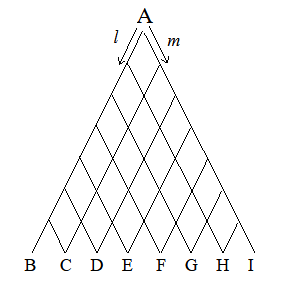
\includegraphics[width=0.95\columnwidth]{img/9.0 triangle.png}
\end{minipage}
\end{figure} 

\begin{thm}
    Фабрика окрашивает кубики в 6 цветов (каждую грань в свой цвет, набор цветов фиксирован). Сколько разновидностей кубиков можно изготовить?
\end{thm}

\begin{thm}
    На окружности даны 10 точек. Сколькими способами можно провести пять непересекающихся отрезков с концами в заданных точках?
\end{thm}

\begin{thm}
    Имеется прямоугольная доска $30 \times 40$. Найдите число прямоугольников, составленных из клеток этой доски.
\end{thm}

\begin{thm}
    У Кости есть $n$ друзей, и каждый день он приглашает некоторых из них в гости так, чтобы компания ни разу не повторялась (в какой-то день он может не пригласить никого). Сколько дней он сможет так делать?
\end{thm}

{\setlength{\intextsep}{2pt}
\begin{figure}[h]
\begin{minipage}{0.55\linewidth}\setlength{\parindent}{1.5em}
    \begin{thm}
    Сколькими способами можно добраться из пункта А
в пункт В по линиям сетки без самопересечений?
    \end{thm}
\end{minipage}
\hfill
\begin{minipage}{0.35\linewidth}\setlength{\parindent}{1.5em}
    A \begin{tabular}{ |m{.1em}|m{.1em}|m{.1em}|m{.1em}|m{.1em}|m{.1em}|m{.1em}|m{.1em}|m{.1em}|c| } 
    \hline
     & & & & & & & & & \\ 
    \hline
    \end{tabular} B
\end{minipage}
\end{figure}}

\begin{thm}
    Сколькими способами можно из последовательности 1, 2, ..., 2$n$ выбрать три числа, образующих арифметическую прогрессию?
\end{thm}

\begin{thm}
    У Вани есть кучка из 2012 морковок. Каждую минуту он произвольным образом делит одну из имеющихся у него кучек на две до тех пор, пока не получит 2012 кучек по одной морковке. При каждом делении Ваня записывает произведение числа морковок в получившихся двух кучках. Чему в результате равна сумма этих произведений?
\end{thm}

\begin{thm}
    Найдите количество клетчатых прямоугольников шахматной доски, содержащих клетку с4.
\end{thm}

\begin{thm}
    Сколько наборов целых чисел удовлетворяют условию:
    \par
    а) $0 < a_1 < a_2 < ... < a_n < n$; \hfill б) $0 \leq a_1 \leq a_2 \leq ... \leq a_n \leq n$? 
\end{thm}

\begin{thm}
    Сколько наборов целых неотрицательных чисел удовлетворяют условию:
    \par
    а) $a_1 + a_2 + ... + a_n = n$; \hfill б) $a_1 + a_2 + ... + a_n \leq n$? 
\end{thm}
\head{Декабрь}{Листок 10. Графы. Уровень 1.}

\section{Подсчёт рёбер, двудольные графы, независимые множества.}

Как уже выводилось ранее, удвоенное количество ребер равно сумме всех степеней вершин графа. Часто идея подсчёта рёбер помогает решить задачу. Одна из идей состоит в подсчете концов рёбер (которая как раз и равна сумме степеней всех вершин). Лемма о рукопожатиях именно так и доказывается. Обобщением этой идеи является подсчёт концов рёбер двумя способами. Часто такая идея применяется, если рассматриваемый граф -- \textit{двудольный}.

\begin{dfn}
    Граф двудольный, если его множество вершин можно разбить на два подмножества так, что все рёбра будут соединять только элементы разных подмножеств.
\end{dfn}

\begin{thm}
    По окончании конкурса бальных танцев, в котором участвовали 7 мальчиков и 8 девочек, каждый назвал количество своих партнеров / партнёрш:3, 3, 3, 3, 3, 5, 6, 6, 6, 6, 6, 6, 6, 6, 6. Не ошибся ли кто--нибудь из них?
\end{thm}

\begin{prf}
    Рассмотрим граф, в котором вершины соответствуют танцорам, и две вершины соединены ребром, если они были партнёрами в танце. Ясно, что такой граф будет двудольным, в одной доле мальчики, в другой -- девочки. Количество партнёров / партнёрш, которое было названо -- это степень соответствующей вершины. Значит, эти степени можно разбить на два подмножества, степени доли мальчиков и степени доли девочек. Ясно, что число концов рёбер доли мальчиков в сумме равно числу концов рёбер доли девочек. Если степень 5 принадлежит одной доле, то к другой доле относятся степени 3 или 6, все они делятся на 3, поэтому сумма степеней одной доли делится на 3, а другой не делится. Следовательно, кто--то ошибся.  
\end{prf}

Часто подсчитывается не число рёбер, а число пар, троек и т.д. рёбер выходящих из одной вершины, как в следующем примере.

\begin{thm}
    Кружок по астрономии проводился в школе 20 раз. На каждое занятие приходило 5 человек. Известно, что никакие 2 школьника не встречались более чем на одном занятии. Доказать, что не менее 20 школьников посетили кружок.
\end{thm}

\begin{prf}
    Предположим, что это не так, и пусть школьников было не более 20. Рассмотрим двудольный граф, в верхней доле которого находятся вершины--школьники, а в нижней находятся вершины--занятия. Соединим их, если школьник посетил соответствующее занятие. Посчитаем число пар школьников двумя способами. С одной стороны их не более $\dfrac{20 \times 19}{2} = 190$. С другой стороны это число равно числу пар рёбер выходящих из вершины в нижней доле (занятия), т.е. их $20 \times (\dfrac{4 \times 5}{2}) = 200$. Противоречие.
\end{prf}

Иногда считается количество ребер, выходящих из какого--либо множества.

\begin{dfn}
    Назовем \textit{независимым} множеством вершин графа такое множество его вершин, что никакие две из них не соединены ребром.
\end{dfn}

\begin{dfn}
    Назовем \textit{доминирующим} множеством такое множество D вершин графа, что любая вершина соединена ребром с вершиной из D.
\end{dfn}

\begin{dfn}
    \textit{Максимальное} независимое множество вершин -- независимое множество вершин, которое становится зависимым при добавлении любой вершины.
\end{dfn}

С помощью подсчёта ребер можно доказать следующее утверждение.

\fbox{\begin{varwidth}{0.95\textwidth}
    \textbf{Теорема.} Если степени всех вершин в графе G не превосходят $l$, то число элементов в любом максимальном независимом множестве не меньше $\dfrac{V}{l + 1}$.
\end{varwidth}}

\textbf{Идеи доказательства.} Если I это максимальное независимое множество, то из I существует ребро
\\ к любой вершине из J -- дополнения к I. Значит $V = |I| + |J| \leq |I| + l |I|$.
\\  
Отсюда уже выводится требуемое неравенство.    


\section{Подсчёт рёбер, двудольные графы, независимые множества.}

Как уже выводилось ранее, удвоенное количество ребер равно сумме всех степеней вершин графа. Часто идея подсчёта рёбер помогает решить задачу. Одна из идей состоит в подсчете концов рёбер (которая как раз и равна сумме степеней всех вершин). Лемма о рукопожатиях именно так и доказывается. Обобщением этой идеи является подсчёт концов рёбер двумя способами. Часто такая идея применяется, если рассматриваемый граф -- \textit{двудольный}.

\begin{dfn}
    Граф двудольный, если его множество вершин можно разбить на два подмножества так, что все рёбра будут соединять только элементы разных подмножеств.
\end{dfn}

\begin{thm}
    По окончании конкурса бальных танцев, в котором участвовали 7 мальчиков и 8 девочек, каждый назвал количество своих партнеров / партнёрш:3, 3, 3, 3, 3, 5, 6, 6, 6, 6, 6, 6, 6, 6, 6. Не ошибся ли кто--нибудь из них?
\end{thm}

\begin{prf}
    Рассмотрим граф, в котором вершины соответствуют танцорам, и две вершины соединены ребром, если они были партнёрами в танце. Ясно, что такой граф будет двудольным, в одной доле мальчики, в другой -- девочки. Количество партнёров / партнёрш, которое было названо -- это степень соответствующей вершины. Значит, эти степени можно разбить на два подмножества, степени доли мальчиков и степени доли девочек. Ясно, что число концов рёбер доли мальчиков в сумме равно числу концов рёбер доли девочек. Если степень 5 принадлежит одной доле, то к другой доле относятся степени 3 или 6, все они делятся на 3, поэтому сумма степеней одной доли делится на 3, а другой не делится. Следовательно, кто--то ошибся.  
\end{prf}

Часто подсчитывается не число рёбер, а число пар, троек и т.д. рёбер выходящих из одной вершины, как в следующем примере.

\begin{thm}
    Кружок по астрономии проводился в школе 20 раз. На каждое занятие приходило 5 человек. Известно, что никакие 2 школьника не встречались более чем на одном занятии. Доказать, что не менее 20 школьников посетили кружок.
\end{thm}

\begin{prf}
    Предположим, что это не так, и пусть школьников было не более 20. Рассмотрим двудольный граф, в верхней доле которого находятся вершины--школьники, а в нижней находятся вершины--занятия. Соединим их, если школьник посетил соответствующее занятие. Посчитаем число пар школьников двумя способами. С одной стороны их не более $\dfrac{20 \times 19}{2} = 190$. С другой стороны это число равно числу пар рёбер выходящих из вершины в нижней доле (занятия), т.е. их $20 \times (\dfrac{4 \times 5}{2}) = 200$. Противоречие.
\end{prf}

Иногда считается количество ребер, выходящих из какого--либо множества.

\begin{dfn}
    Назовем \textit{независимым} множеством вершин графа такое множество его вершин, что никакие две из них не соединены ребром.
\end{dfn}

\begin{dfn}
    Назовем \textit{доминирующим} множеством такое множество D вершин графа, что любая вершина соединена ребром с вершиной из D.
\end{dfn}

\begin{dfn}
    \textit{Максимальное} независимое множество вершин -- независимое множество вершин, которое становится зависимым при добавлении любой вершины.
\end{dfn}

С помощью подсчёта ребер можно доказать следующее утверждение.

\fbox{\begin{varwidth}{0.95\textwidth}
    \textbf{Теорема.} Если степени всех вершин в графе G не превосходят $l$, то число элементов в любом максимальном независимом множестве не меньше $\dfrac{V}{l + 1}$.
\end{varwidth}}

\textbf{Идеи доказательства.} Если I это максимальное независимое множество, то из I существует ребро
\\ к любой вершине из J -- дополнения к I. Значит $V = |I| + |J| \leq |I| + l |I|$.
\\  
Отсюда уже выводится требуемое неравенство.    
\head{Ноябрь}{Листок 10. Графы. Теория 1.}

\epigraph{\textit{«Бамбук -- дерево, ёжик -– дерево, ёжики с бамбуком –- лес...»}}

\textbf{\textit{Напоминание.}} Связный граф, не имеющий циклов, называется \textit{деревом}.

\fbox{\begin{varwidth}{0.95\textwidth}
    \textbf{\textit{Лемма.}} Граф является деревом тогда и только тогда, когда каждые две его вершины соединены ровно одним путём с различными ребрами.
\end{varwidth}}

\textit{\underline{Замечание}}: иногда дерево определяют именно как граф, в котором любые две вершины соединены ровно одним путём с различными ребрами (т.е. простым путём).

\begin{dfn}
    Вершина, из которой выходит только одно ребро, называется \textit{висячей}.
\end{dfn}

\fbox{\begin{varwidth}{0.95\textwidth}
    \textbf{\textit{Лемма о висячей вершине.}} В любом дереве найдётся висячая вершина.
\end{varwidth}}

\begin{dok}
    Выберем произвольную вершину А и рассмотрим какое--нибудь выходящее из этой вершины ребро. Пусть это ребро АВ. Если из вершины В не выходит других рёбер, то эта вершина –- искомая. В противном случае отметим ребро АВ и продолжим наш путь по любому неотмеченному ребру, выходящему из вершины B и так далее. Заметим, что в строящемся таким образом пути ни одна вершина не встречается дважды, в противном случае получился бы цикл, а дерево циклов не имеет. Поэтому при наличии неотмеченных рёбер мы будем каждый раз переходить в новую вершину, а их конечное число. Следовательно, в конце концов наш путь закончится. Но закончиться он может только в висячей вершине.
\end{dok}

\fbox{\begin{varwidth}{0.95\textwidth}
    \textbf{\textit{Утверждение.}} Число вершин дерева на единицу больше числа его рёбер.
\end{varwidth}}

\begin{thm}
    В стране Древляндии 2012 городов, некоторые из которых соединены дорогами. При этом любые два города соединяет ровно один маршрут. Сколько в этой стране дорог?
\end{thm}

\begin{prf}
    Поскольку любые два города соединяет ровно один маршрут (т.е. путь), то граф дорог этой страны – дерево. Поэтому рёбер (дорог) на единицу меньше, чем вершин. Следовательно вершин 2011.
\end{prf}

\begin{dfn}
    Граф О называется \textit{остовом} связного графа G, если О имеет те же вершины, что и G, получается из G удалением некоторых рёбер, и является деревом.
\end{dfn}

\fbox{\begin{varwidth}{0.95\textwidth}
    \textbf{\textit{Лемма об остове.}} Любой связный граф имеет остов.
\end{varwidth}}

\begin{dok}
    Если граф уже является деревом, то в качества остова можно выбрать его самого. Пусть данный граф не является деревом. Тогда докажем, что в любом таком графе мы можем удалить одно ребро без потери связности. Действительно, если этот граф не дерево, то в нём есть цикл. Удалим в цикле одно ребро. Очевидно, что граф останется связным. Поскольку если две вершины были соединены путём, не проходящим через удалённое ребро, то для них ничего не изменилось. Если же путь проходил через удалённое ребро, то заменим это ребро путём по оставшемуся куску цикла. Следовательно, путь восстановлен и граф остался связным. Таким образом, можно удалять по одному ребру до тех пор, пока граф не станет деревом. Но тогда мы получим искомый остов.
\end{dok}

\begin{figure}[H]
\begin{minipage}{0.65\linewidth}\setlength{\parindent}{1.5em}
    \begin{ques}
     Может ли граф иметь несколько остовов?
    \end{ques}

    \begin{thm}
    Рома и Саша стирают у фигуры, приведённой на рисунке по одной стороне квадратиков. Нельзя стирать вершины квадратиков и сторону так, чтобы фигура распалась на две несвязные части. Кто выигрывает в эту игру, если начинает Рома?
    \end{thm}
\end{minipage}
\hfill
\begin{minipage}{0.3\linewidth}

        \begin{tabular}{ | m{0em} | m{0em} | m{0em} | m{0em} | m{0em} | m{0em} | m{0em} | m{0em} | } 
    \hline
   &  &  &  &  &  &  &  \\ 
     \hline
   &  &  &  &  &  &  &  \\ 
    \hline
   &  &  &  &  &  &  &  \\ 
    \hline
   &  &  &  &  &  &  &  \\ 
    \hline
   &  &  &  &  &  &  &  \\ 
    \hline
\end{tabular}
    
\end{minipage}
\end{figure} 

\begin{prf}
    У данной фигуры $8 \times 6 + 9 \times 5 = 93$ стороны маленьких квадратиков (ребер графа) и $6 \times 9 = 54$ вершины. Не получится стереть сторону лишь тогда, когда граф станет деревом. Но тогда при 54 вершинах должно будет остаться 53 ребра. Поэтому при любых ходах стереть можно ровно 40 отрезков и выиграет Саша, поскольку именно он делает чётные ходы. \textbf{\textit{Ответ}}: выиграет Саша
\end{prf}
\head{Декабрь}{Листок 10. Графы. Теория 3.}

\section{Эйлеровы и гамильтоновы обходы. Ориентированные графы.}

\begin{dfn}
    Граф называется \textit{эйлеровым}, если в нем существует цикл, проходящий по всем ребрам по одному разу, так называемый \textit{эйлеров цикл}. \textit{Полуэйлеров} (или \textit{почти эйлеров}) граф -- граф, в котором есть путь, проходящий по одному разу по каждому ребру.
\end{dfn}

\textit{\underline{Замечание}}: в частности любой эйлеров граф является почти эйлеровым, т.к. любой цикл является путём. Примером почти эйлеровых графов являются фигуры, которые можно нарисовать, не отрывая карандаша от бумаги и не проводя карандаш повторно по каким-либо линиям. 

\fbox{\begin{varwidth}{0.95\textwidth}
    \textbf{Теорема Эйлера (критерий эйлеровости графа)}. Граф эйлеров тогда и только тогда, когда он связен, и все его вершины имеют чётную степень. Граф полуэйлеров тогда и только тогда, когда он связен и имеет не более двух вершин с нечётной степенью.
\end{varwidth}}

\begin{dfn}
    Граф называется \textit{гамильтоновым}, если в нём существует замкнутый путь, проходящий через все вершины ровно по одному разу. Такой путь, соответственно, называют \textit{гамильтоновым} \textit{циклом}.
\end{dfn}

% \begin{figure}[H]
% \begin{minipage}{0.65\linewidth}\setlength{\parindent}{1.5em}
%     Многие головоломки сводятся к эйлеровости или гамильтоновости определенных графов. Эйлер придумал свою теорему в 1736 году в связи с задачей об обходе кенигсбергских мостов. Именно с теоремы Эйлера теория графов отсчитывает свою историю. Гамильтоновы путь, цикл и граф названы в честь ирландского математика сэра Уильяма Гамильтона, который в 1859 году впервые определил эти классы, исследовав задачу «кругосветного путешествия» по додекаэдру, узловые вершины которого символизировали крупнейшие города Земли, а рёбра – соединяющие их дороги. Играющий должен обойти все города и вернуться в исходный. 
% \end{minipage}
% \hfill
% \begin{minipage}{0.3\linewidth}
%     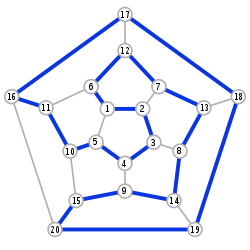
\includegraphics[width=0.95\columnwidth]{img/10.2 1 pyat.png}
% \end{minipage}
% \end{figure} 

\begin{wrapfigure}{R}{0.35\textwidth}
\centering
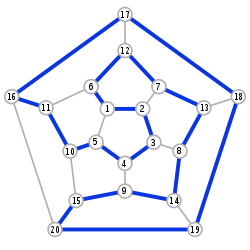
\includegraphics[width=0.3\textwidth]{img/10.2 1 pyat.png}
\end{wrapfigure}

Многие головоломки сводятся к эйлеровости или гамильтоновости определенных графов. Эйлер придумал свою теорему в 1736 году в связи с задачей об обходе кенигсбергских мостов. Именно с теоремы Эйлера теория графов отсчитывает свою историю. Гамильтоновы путь, цикл и граф названы в честь ирландского математика сэра Уильяма Гамильтона, который в 1859 году впервые определил эти классы, исследовав задачу «кругосветного путешествия» по додекаэдру, узловые вершины которого символизировали крупнейшие города Земли, а рёбра – соединяющие их дороги. Играющий должен обойти все города и вернуться в исходный. Справедливости ради следует отметить, что уже до этого была задача, сводящаяся к гамильтоновости некоторого графа, а именно задача обхода конем всех полей шахматной доски с возвращением в исходную клетку. Эта задача была в своё время успешно решена Эйлером. На рисунке изображен граф додекаэдра Гамильтона.

\begin{figure}[H]\begin{minipage}{0.3\linewidth}
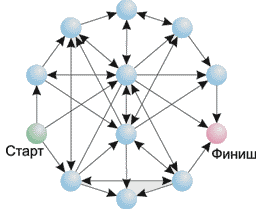
\includegraphics[width=0.95\columnwidth]{img/10.2curse.png}
\end{minipage}
\hfill
\begin{minipage}{0.69\linewidth}\setlength{\parindent}{1.5em}
    \begin{dfn}
    Пусть $n$ -- количество вершин в данном графе. Если степень каждой вершины не менее, чем $\dfrac{n}{2}$, то граф называется \textit{графом Дирака}.
    \end{dfn}
    \begin{ques}
        Почему граф Дирака связен?
    \end{ques} 
    (На рисунке изображён граф из задачи поиска гамильтонова пути с помощью ДНК--вычислений.)
    \\
    Для гамильтоновости графов в отличие от эйлеровости не найдено простых критериев. Тем не менее существует много достаточных условий. Приведём некоторые из них.
\end{minipage}
\end{figure}

\fbox{\begin{varwidth}{0.95\textwidth}
    \textbf{Теорема Поша.} Пусть граф имеет p вершин, где $p \geq 3$. Если для всякого $n$ такого, что $1 \leq n \leq \dfrac{p - 1}{2}$, число вершин со степенями, не превосходящими $n$, меньше чем $n$, и для нечётного $p$ количество вершин степени $\dfrac{p - 1}{2}$ не превосходит $\dfrac{p - 1}{2}$, то такой граф гамильтонов.
    \\
    \textbf{Теорема Оре.} Если граф имеет $p$ вершин, где $p > 2$ и сумма степеней несмежных вершин не меньше $p$, то граф гамильтонов. 
    \\ 
    \textbf{Теорема Дирака.} Если граф имеет $p$ вершин, где $p > 2$ и степень любой вершины не меньше $\dfrac{p}{2}$, то граф гамильтонов.
\end{varwidth}}

\newpage

\begin{ques}
    Является ли дерево эйлеровым графом?
\end{ques}

\begin{ques}
    Является ли дерево гамильтоновым графом?
\end{ques}

\begin{dfn}
    Граф называется \textit{двусвязным}, если между любыми двумя вершинами существует два непересекающихся по вершинам (кроме начала и конца) пути.
\end{dfn}

\textit{\textbf{Утверждение.}} Гамильтонов граф двусвязен.

\begin{dfn}
    \textit{Тэта-графом} называется граф из двух вершин степени 3 и трёх непересекающихся простых путей, соединяющих их, причём длина каждого из путей не меньше 2.
\end{dfn}

\fbox{\begin{varwidth}{0.95\textwidth}
    \begin{thrm}
        Каждый негамильтонов двусвязный граф содержит тэта--подграф.
    \end{thrm}
\end{varwidth}}

Задачи, в которых нужно доказать отсутствие гамильтонова цикла, часто сводятся к поиску инварианта или какой-нибудь величины на вершинах, которая известным образом изменяется при переходе от вершины к смежной вершине. Как, например, шахматная раскраска в следующем примере.

\begin{thm}
    Докажите, что шахматный конь не может обойти доску 5 на 5 и вернуться в исходную клетку.
\end{thm}

\begin{prf}
    Каждым ходом конь встаёт на клетку другого цвета. Так как всего ходов 25 -- нечётное число, то последним ходом он должен встать на клетку, не совпадающую по цвету с начальной. Противоречие.
\end{prf}

\begin{dfn}
    Граф, в котором рёбра снабжены стрелками, называется ориентированным. Полный граф, в котором каждое ребро снабжено ориентацией (стрелкой), называется \textit{полным ориентированным графом }или \textit{турниром}.
\end{dfn}

\begin{dfn}
    \textit{Исходящей степенью} вершины в ориентированном графе называется количество рёбер, выходящих из данной вершины. \textit{Входящей степенью} вершины в ориентированном графе называется количество рёбер, входящих в данную вершину.
\end{dfn}
\hfill \break
Заметим следующий общий факт. Так как каждое ориентированное ребро имеет одно начало и один конец, то сумма всех исходящих степеней вершин равна количеству рёбер. Аналогично каждое ребро имеет один конец, поэтому сумма входящих степеней вершин равна количеству рёбер. Потому сумма исходящих степеней вершин равна сумме входящих степеней вершин.

\begin{thm}
    В однокруговом турнире по настольному теннису каждый участник одержал четыре победы. Сколько человек участвовало в турнире? (Ничьих в теннисе не бывает).
\end{thm}

\begin{prf}
    Обозначим участников за вершины графа. Если участник A выиграл у участника B, поставим стрелку от A к B. Переформулировка на язык графов: «В полном ориентированном графе из каждой вершины выходит четыре ребра. Сколько в нём вершин?».
    \\
    Пусть всего в графе $x$ вершин, у каждой из которых исходящая степень 4. Сумма исходящих степеней вершин -- $4x$, сумма входящих -- такая же. Так как общая степень каждой вершины одна и та же и равна $x – 1$, а исходящая равна 4, то входящая степень у всех вершин тоже одинакова. Значит, она тоже равна 4. Отсюда $x
    – 1 = 8$, и в турнире принимало участие 9 человек.
\end{prf}
\head{Декабрь}{Переводная самостоятельная работа. Уровень 1 $\Rightarrow$ уровень 2.}

\section{Подсчёт рёбер, двудольные графы. Обходы.}

\begin{figure}[H]
\begin{minipage}{0.19\linewidth}
    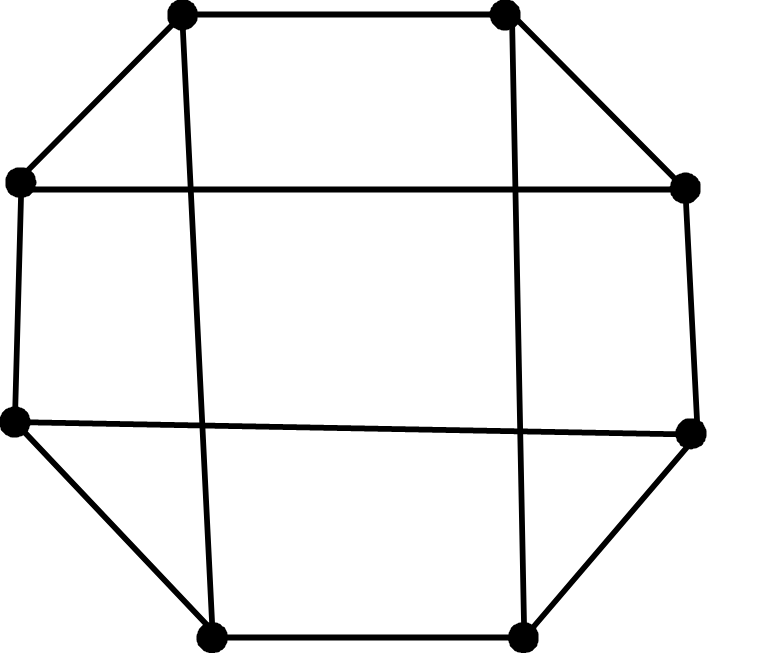
\includegraphics[width=0.95\columnwidth]{img/10.4.0 img1.png}
\end{minipage}
    \hfill
\begin{minipage}{0.8\linewidth}
    \begin{thm}
        Является ли граф, приведённый на рисунке, двудольным?
    \end{thm}
    \begin{thm}
        На конкурсе по математике было 20 задач. На разбор пришло 20 школьников. Известно, что каждый школьник решил ровно две задачи и каждую задачу решило ровно два школьника. Докажите, что можно так организовать разбор задач, что каждую задачу расскажет решивший её школьник.
    \end{thm}
\end{minipage}
\end{figure}

\begin{figure}[H]
\begin{minipage}{0.6\linewidth}
    \begin{thm}
        На рисунке изображён план дома. Линиями отмечены стены. (см. рис.) Можно ли провести по дому освещение (протянуть один провод) так, чтобы при этом просверлить каждую стену ровно один раз?
    \end{thm}
    \begin{thm}
        В одном учреждении каждый сотрудник выписывает две газеты, каждую газету выписывают пять человек, каждую пару газет выписывает только один человек. Сколько человек в учреждении и сколько они выписывают газет?
    \end{thm}
\end{minipage}
    \hfill
\begin{minipage}{0.39\linewidth}
    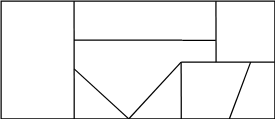
\includegraphics[width=0.95\columnwidth]{img/10.4.0 img2.png}
\end{minipage}
\end{figure}

\begin{thm}
    Докажите, что если граф двудольный, то все его циклы состоят из чётного числа рёбер.
\end{thm}

\begin{thm}
    Докажите, что если в графе все циклы чётной длины, то этот граф -- двудольный.
\end{thm}

\begin{thm}
    В стране Карликании 11 городов. Известно, что среди любых трёх из них хотя бы двое ещё не соединены авиалинией. Докажите, что в стране не более 30 авиалиний.
\end{thm}

\begin{thm}
    Докажите, что независимое множество максимально тогда и только тогда, когда оно доминирующее.
\end{thm}

\begin{thm} $^*$
    Докажите теорему из листка с теорией, воспользовавшись подсказкой.
\end{thm}

\begin{thm}
    В шахматном турнире в один круг участвуют 11 шахматистов. В настоящее время среди любых трёх из них хотя бы двое еще не сыграли. Доказать, что сыграно не более 30 партий.
\end{thm}

\begin{thm}
В классе каждый мальчик дружит ровно с двумя девочками, а девочка -- ровно с тремя мальчиками. Ещё известно, что в классе 31 пионер и 19 парт. Сколько человек в классе?
\end{thm}

\begin{thm}
    В народной дружине 100 человек. В каждый вечер на дежурство выходят трое. Докажите, что нельзя составить график дежурств таким образом, что любые два человека будут дежурить вместе ровно один раз.
\end{thm}

\begin{thm}
    Кружок по астрономии проводился в школе 20 раз. На каждое занятие приходило 6 человек. Известно, что никакие два школьника не встречались более чем на одном занятии. Доказать, что не менее 21 школьника посетили кружок.
\end{thm}

\begin{figure}[H]
    \begin{minipage}{0.89\linewidth}\setlength{\parindent}{1.5em}
        \begin{thm}
             В некоторые 16 клеток доски 8×8 поставили по ладье. Какое наименьшее количество пар бьющих друг друга ладей могло при этом оказаться?
        \end{thm}
        \begin{thm}
            На рисунке изображён план парка и его окрестностей, линиями отмечены заборы. (см. рис.) Можно ли прогуляться по парку так, чтобы при этом перелезть через каждый забор ровно один раз?
        \end{thm}
    \end{minipage}
\hfill
    \begin{minipage}{0.1\linewidth}
        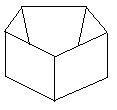
\includegraphics[width=0.95\columnwidth]{img/10.4 figure.png}
    \end{minipage}
\end{figure}

\begin{thm}
    В футбольном турнире участвует 20 команд. После того, как все команды провели по две игры, организаторы турнира решили разбить их на три дивизиона, но так, чтобы в одном дивизионе не было команд, уже игравших друг с другом. Всегда ли они смогут это сделать? (Подсказка. Вспомните теорему о циклических графах)
\end{thm}

\begin{thm}
    На $n$ карточках с двух сторон написаны числа от 1 до $n$ по два раза каждое. Докажите, что карточки можно положить на стол так, чтобы сверху каждое из чисел было написано ровно один раз.
\end{thm}

\begin{thm} $^*$
    В некоторой стране из каждого города выходит по три железные дороги. Две компании хотят их все приватизировать. Антимонопольный комитет требует, чтобы из каждого города выходили дороги обеих компаний. Докажите, что компании могут договориться так, чтобы требование антимонопольного комитета было выполнено.
\end{thm}

\begin{thm}
    Сварщик варит решетку размером 4×4 из кусков ломаных. Сможет ли он это сделать, если у него есть а) 5 ломаных длины 8; б) 8 ломаных длины 5? \textit{(Форма ломаных может быть различной)}
\end{thm}

\end{document}


